%-----------------------------------------------
%  Engineer's & Master's Thesis Template
%  Copyleft by Artur M. Brodzki & Piotr Woźniak
%  Warsaw University of Technology, 2019-2022
%-----------------------------------------------

\documentclass[
    bindingoffset=5mm,  % Binding offset
    footnoteindent=3mm, % Footnote indent
    hyphenation=true    % Hyphenation turn on/off
]{src/wut-thesis}

\graphicspath{{tex/img/}} % Katalog z obrazkami.
\addbibresource{bibliografia.bib} % Plik .bib z bibliografią

%-------------------------------------------------------------
% Wybór wydziału:
%  \facultyeiti: Wydział Elektroniki i Technik Informacyjnych
%  \facultymeil: Wydział Mechaniczny Energetyki i Lotnictwa
% --
% Rodzaj pracy: \EngineerThesis, \MasterThesis
% --
% Wybór języka: \langpol, \langeng
%-------------------------------------------------------------
\facultyeiti    % Wydział Elektroniki i Technik Informacyjnych
\EngineerThesis % Praca inżynierska
\langpol % Praca w języku polskim

\begin{document}

%------------------
% Strona tytułowa
%------------------
\instytut{Automatyki i Informatyki Stosowanej}
\kierunek{Informatyka}
\specjalnosc{Inżynieria Oprogramowania}
\title{
    Zastosowanie architektur mikroserwisowych\\
    w tworzeniu skalowalnych aplikacji webowych\\ 
    na przykładzie aplikacji do obsługi zamówień restauracyjnych
}
% Title in English for English theses
% In English theses, you may remove this command
\engtitle{
    Application of microservice architectures \\
    in creating scalable web applications:\\
    a case study of a restaurant order management application
}
% Title in Polish for English theses
% Use it only in English theses
\poltitle{
    Zastosowanie architektur mikroserwisowych\\
    w tworzeniu skalowalnych aplikacji webowych\\ 
    na przykładzie aplikacji do obsługi zamówień restauracyjnych
}
\author{Bartłomiej Patryk Rasztabiga}
\album{304117}
\promotor{mgr inż. Zbigniew Szymański}
\date{\the\year}
\maketitle

%-------------------------------------
% Streszczenie po polsku dla \langpol
% English abstract if \langeng is set
%-------------------------------------
\cleardoublepage % Zaczynamy od nieparzystej strony
\abstract

Praca prezentuje proces projektowania oraz implementacji systemu informatycznego opartego na architekturze mikroserwisowej, służącego do obsługi zamówień restauracyjnych w kontekście dostaw jedzenia. Został on zaimplementowany jako dwie warstwy: kliencka (aplikacja internetowa działająca w przeglądarce) oraz serwerowa.

Kolejne etapy, zrealizowane w ramach poniższej pracy inżynierskiej, to analiza wymagań funkcjonalnych oraz niefunkcjonalnych, podział systemu na mikroserwisy, implementacja aplikacji odpowiedzialnych za warstwę prezentacji, logikę biznesową oraz zarządzanie warstwą danych. Zwieńczeniem pracy było przetestowanie systemu pod kątem skalowalności i wydajności.

Analiza wymagań została poprzedzona omówieniem architektury mikroserwisowej oraz wzorców i technik pomocnych w tworzeniu skalowalnych aplikacji webowych.

W trakcie opisywania implementacji systemu omówiono na bieżąco używane narzędzia i technologie, wraz z przykładami ich zastosowania w systemie. Zastosowano projekcyjne bazy danych w technologii MongoDB. Warstwa logiki biznesowej to mikroserwisy napisane w języku Kotlin, przy użyciu Spring Framework oraz Axon Framework, udostępniające interfejs REST. Zdarzenia są przechowywane i dostarczane pomiędzy serwisami przy pomocy narzędzia Axon Server. Warstwa prezentacji to aplikacja webowa, uruchamiana w przeglądarce klienckiej, przy wykorzystaniu bibliotek Remix i React.

Testowanie systemu składało się z przygotowania oraz przeprowadzanie testów jednostkowych, integracyjnych, akceptacyjnych oraz wydajnościowych.

W podsumowaniu przedstawiono wnioski z testów wydajności prezentujące skalowalność systemu oraz możliwości dalszego jego rozwoju.

\keywords architektura mikroserwisowa, skalowalnosć, aplikacje webowe, Kotlin, Spring, Axon, MongoDB, React

%----------------------------------------
% Streszczenie po angielsku dla \langpol
% Polish abstract if \langeng is set
%----------------------------------------
\clearpage
\secondabstract

The thesis presents the process of designing and implementing an information system based on microservices architecture for managing restaurant orders in the context of food delivery. It has been implemented as two layers: client (a web application operating in a browser) and server.

The subsequent stages, realized within this engineering thesis, include the analysis of functional and non-functional requirements, division of the system into microservices, implementation of applications responsible for the presentation layer, business logic, and data layer management. The culmination of the work was testing the system in terms of scalability and performance.

The requirements analysis was preceded by a discussion of the microservices architecture and patterns and techniques helpful in creating scalable web applications.

During the description of the system implementation, the tools and technologies used were discussed on an ongoing basis, along with examples of their application in the system. Projection databases in MongoDB technology were used. The business logic layer consists of microservices written in Kotlin, using the Spring Framework and Axon Framework, providing a REST interface. Events are stored and delivered between services using the Axon Server tool. The presentation layer is a web application, launched in the client's browser, using Remix and React libraries.

Testing of the system consisted of preparing and conducting unit, integration, acceptance, and performance tests.

The summary presents conclusions from performance tests showing the scalability of the system and possibilities for its further development.

\secondkeywords microservices architecture, scalability, web applications, Kotlin, Spring, Axon, MongoDB, React

\pagestyle{plain}

%--------------
% Spis treści
%--------------
\cleardoublepage % Zaczynamy od nieparzystej strony
\tableofcontents

%------------
% Rozdziały
%------------
\cleardoublepage % Zaczynamy od nieparzystej strony
\pagestyle{headings}

\clearpage % Rozdziały zaczynamy od nowej strony.
\section{Wstęp}

\subsection{Motywacja}

Wybór tematu pracy dyplomowej został podyktowany chęcią pogłębienia wiedzy oraz zaprezentowania technik tworzenia skalowalnych systemów mikroserwisowych na podstawie konkretnej aplikacji.

Wybraną przez Autora dziedziną do tego celu jest branża gastronomiczna. W ostatnich latach, wraz z rozwojem techniki, zaczęło powstawać wiele aplikacji służących do zamawiania jedzenia z restauracji. Aplikacje te cieszą się ogromną popularnością, więc ich twórcy muszą zapewnić odpowiednią skalowalność systemu, aby móc obsłużyć duży ruch. Jednym z rozwiązań tego problemu jest zastosowanie skalowalnych architektur, np. architektury mikroserwisowej.

Architektura mikroserwisowa jest jednym z najbardziej innowacyjnych podejść do tworzenia aplikacji webowych. W ostatnich latach zyskała ona na popularności, a jej zalety są doceniane przez coraz większą liczbę programistów. Wymaga ona jednak zupełnie innego podejścia niż architektura monolityczna, która jest najczęściej stosowana w aplikacjach tego typu. Różnice wynikają np. z innego podejścia do transakcyjności, synchronizacji danych oraz komunikacji między komponentami.

W pracy dyplomowej Autor prezentuje przykład aplikacji webowej zbudowanej zgodnie z najlepszymi praktykami architektury mikroserwisowej. Aplikacja ta będzie służyła do obsługi zamówień restauracyjnych z trzech perspektyw: klienta, restauracji oraz dostawcy.

TODO

\subsection{Cel pracy}

XXX

\subsection{Charakterystyka problemu}

XXX

\subsection{Przegląd podobnych rozwiązań}

XXX

\subsection{Struktura pracy}

XXX

         % Wygodnie jest trzymać każdy rozdział w osobnym pliku.
\clearpage
\section{Techniki tworzenia skalowalnych aplikacji webowych}

Przed przystąpieniem do implementacji projektu inżynierskiego, istotne jest zrozumienie technik i narzędzi stosowanych w tworzeniu nowoczesnych, skalowalnych aplikacji webowych. Opisane poniżej elementy znalazły zastosowanie w ramach niniejszej pracy.

\subsection{Architektura mikroserwisowa}

Przez lata pojawiło się wiele definicji architektury oprogramowania. Dobrze pojęcie to obrazują Panowie Bass, Clements i Kazman podając w 2003 roku \cite{bass2012software}, że

\begin{displayquote}
\emph{Architektura oprogramowania programu lub systemu informatycznego jest strukturą lub zbiorem struktur tego systemu, obejmującym elementy oprogramowania, widoczne dla pozostałych elementów oprogramowania oraz zależności między nimi.}
\end{displayquote}

Architektura mikroserwisowa to podejście do strukturyzacji aplikacji jako zbiór niewielkich, niezależnych usług, które komunikują się ze sobą przy użyciu standardowych protokołów komunikacji synchronicznej, takich jak HTTP/gRPC \cite{grpc} lub asynchronicznych kolejek komunikatów, np. RabbitMQ \cite{rabbitmq}/Apache Kafka \cite{kafka}. Każdy mikroserwis jest odpowiedzialny za wykonanie określonej funkcjonalności lub usługi i może być rozwijany, wdrażany oraz zarządzany niezależnie od innych. Ta architektura zapewnia wysoką skalowalność i elastyczność, umożliwiając łatwe wprowadzanie zmian i adaptację do zmieniających się wymagań. Mikroserwisy przechowujące dane często mają swoje własne bazy danych, co zwiększa ich niezależność i izolację od innych części systemu.

\begin{figure}[!h]
    \centering 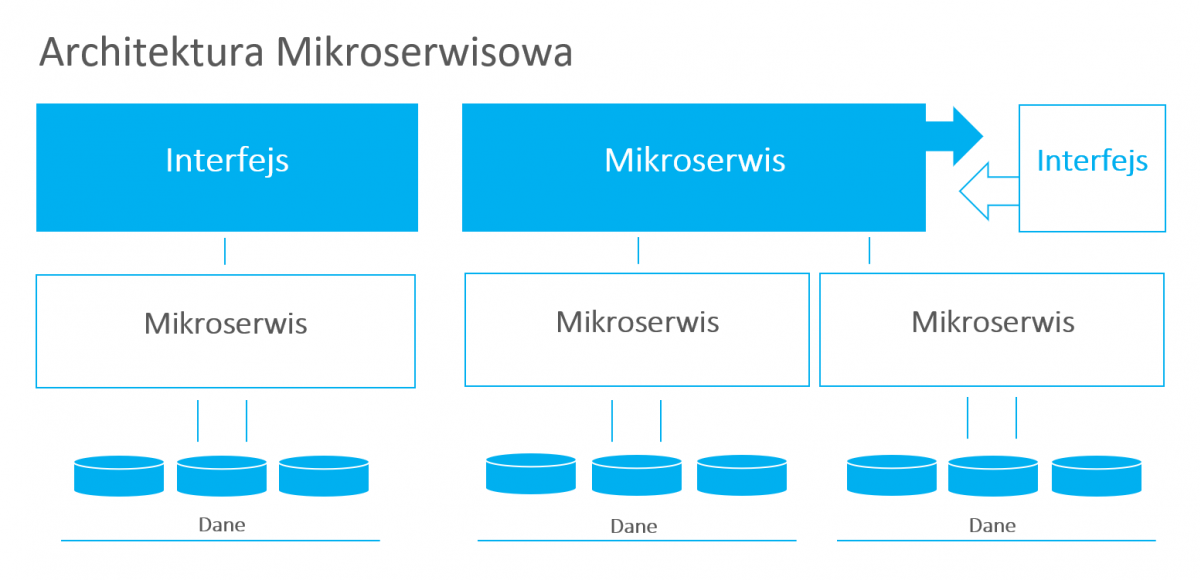
\includegraphics[width=1.0\linewidth]{mikroserwisy.png}
    \caption{Reprezentacja graficzna systemu o architekturze mikroserwisowej \cite{rys1}}
\end{figure}


Główną konsekwencją zastosowania takiej architektury, jest możliwości niezależnego poziomego skalowania każdego komponentu systemu, ponieważ każdy serwis jest osobną jednostką wdrożeniową (np. kontenerem).

Z powodu konieczności komunikacji między elementami systemu, często utrudnione jest zastosowanie spójności natychmiastowej, znanej np. z relacyjnych baz danych. W systemach takich stosowana jest tzw. spójność ostateczna (ang. "eventual consistency") \cite{eventual_consistency}. Powoduje ona, że najnowszy odczyt nie gwarantuje otrzymania danych wynikających z najnowszego zapisu. Utrudnia to m.in. tworzenie interfejsów graficznych dla użytkowników końcowych oraz testowanie aplikacji.

Architektura mikroserwisowa sprzyja tworzeniu systemów o wysokiej niezawodności i dostępności. Uruchamiając wielokrotne instancje poszczególnych serwisów, system staje się odporny na chwilowe awarie. Umożliwia to rozłożenie ruchu pomiędzy instancje.

\begin{longtable}{| m{0.2\linewidth} | m{0.4\linewidth} | m{0.4\linewidth} |}
    \caption{Porównanie architektur: mikroserwisowej i monolitycznej.}
    \label{table:architektura_porownanie} \\

    \hline
    Aspekt & Architektura mikroserwisowa & Architektura monolityczna \\ \hline\hline \endfirsthead \endfoot
    \hline \endlastfoot

    Struktura & Podzielona na mniejsze, niezależne usługi. & Jednolita aplikacja, gdzie wszystkie funkcje są ściśle powiązane i działają jako jedna jednostka. \\ \hline
    Skalowalność & Wysoka; poszczególne mikroserwisy mogą być skalowane niezależnie. & Ograniczona; skalowanie często oznacza konieczność skalowania całej aplikacji. \\ \hline
    Zarządzanie & Możliwość niezależnego zarządzania, rozwijania i wdrażania poszczególnych mikroserwisów. & Zarządzanie całością aplikacji odbywa się centralnie. \\ \hline
    Bazy danych & Każdy mikroserwis może mieć własną bazę danych, zwiększając izolację i niezależność. & Zazwyczaj jedna baza danych dla całej aplikacji. \\ \hline
    Złożoność & Większa złożoność w zarządzaniu i koordynacji między serwisami. & Mniejsza złożoność, ponieważ wszystkie komponenty są w jednym miejscu. \\ \hline
    Odporność na awarie & Wysoka; awaria jednego mikroserwisu zazwyczaj nie wpływa na cały system. & Niższa; awaria w jednym miejscu może wpłynąć na całą aplikację. \\ \hline
    Aktualizacje & Możliwość aktualizowania poszczególnych mikroserwisów niezależnie, bez wpływu na resztę systemu. & Aktualizacje wymagają zwykle zatrzymania i aktualizacji całej aplikacji. \\ \hline
    Komunikacja & Używa lekkich protokołów komunikacyjnych, takich jak HTTP/gRPC, kolejki komunikatów. & Komunikacja wewnętrzna jest mniej skomplikowana, ponieważ wszystko jest częścią jednego systemu. \\ \hline
    Rozwój i utrzymanie	& Może być bardziej skomplikowany ze względu na większą liczbę komponentów i ich niezależność. & Prostsze do zarządzania, dopóki aplikacja nie staje się zbyt duża. \\ \hline
    Spójność danych & Często stosuje model „eventual consistency”, co może komplikować pewne aspekty działania aplikacji. & Łatwiejsza do osiągnięcia spójność danych dzięki centralnej bazie danych. \\ \hline
    Niezawodność  & Każdy serwis może być uruchamiany w wielu instancjach, co zwiększa niezawodność i dostępność.		 & Zależy od pojedynczej instancji aplikacji, co może ograniczać niezawodność.
    \\ \hline
\end{longtable}

Architektura mikroserwisowa jest preferowana do tworzenia skalowalnych aplikacji webowych ze względu na jej zdolność do niezależnego skalowania poszczególnych usług i większą odporność na awarie, co zapewnia elastyczność, niezawodność i szybkość adaptacji do zmieniających się potrzeb.

\subsection{Skalowalność}

Skalowanie usług jest ważnym aspektem w projektowaniu i utrzymaniu aplikacji internetowych, zwłaszcza w kontekście rosnącego zapotrzebowania na usługi danej aplikacji, spowodowanego np. wzrostem liczby użytkowników. W kontekście systemów informatycznych, skalowanie może być realizowane zarówno w sposób poziomy, jak i pionowy.

Skalowanie Poziome: Oznacza dodawanie większej liczby instancji serwisu do obsługi rosnącego obciążenia. W przypadku mikroserwisów, indywidualne serwisy mogą być skalowane niezależnie, co pozwala na zwiększenie wydajności systemu bez konieczności modyfikowania całej architektury. W rozwiązaniach chmurowych takie skalowanie jest bardzo często automatyczne - odpowiednie mechanizmy uruchamiają kolejne instancje serwisów na podstawie zużycia ich zasobów lub np. liczby żądań na sekundę.

Skalowanie Pionowe: Polega na zwiększaniu zasobów (np. CPU, pamięci) w istniejącej instancji serwisu. W architekturze mikroserwisowej jest to mniej powszechne, ponieważ główny nacisk kładzie się na elastyczność i skalowalność poziomą. Skalowanie takie jest bardzo popularne w systemach o architekturze monolitycznej, ponieważ często jest to jedyna opcja na zwiększenie wydajności rozwiązania bez poważnych zmian w architekturze.

Architektura mikroserwisowa umożliwia efektywne skalowanie dzięki izolacji poszczególnych serwisów, co umożliwia ich niezależne zarządzanie, rozwój i skalowanie w zależności od indywidualnych potrzeb i zapotrzebowania. Dzięki temu możliwe jest efektywne zarządzanie zasobami i optymalizacja wydajności systemu.

Tworząc rozproszone systemy przetwarzające dane, należy pamiętać o tzw. twierdzeniu Brewera o CAP.

\begin{figure}[!h]
    \centering 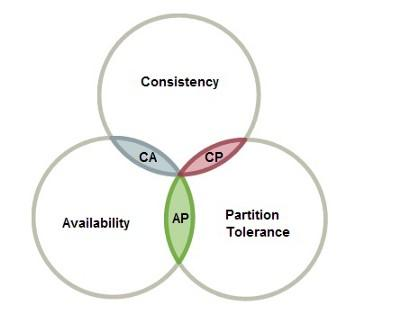
\includegraphics[width=0.3\linewidth]{cap.jpg}
    \caption{Reprezentacja graficzna twierdzenia CAP \cite{rys2}}
\end{figure}

Twierdzenie CAP, odnosi się do trzech podstawowych właściwości, które mogą być gwarantowane w systemach rozproszonych: spójność (Consistency), dostępność (Availability) oraz odporność na rozbicia (Partition Tolerance). Stwierdza ono, że system rozproszony może zapewnić jednocześnie tylko dwie z tych trzech właściwości. Decyzje dotyczące skalowania i zarządzania danymi muszą uwzględniać kompromisy między spójnością, dostępnością i odpornością na rozbicia.

\subsection{Architektura zorientowana na zdarzenia}

Architektura zorientowana na zdarzenia (Event-Driven Architecture, EDA) to podejście, w którym przepływ działania systemu jest sterowany przez zdarzenia - zazwyczaj oznacza to, że działania w systemie są wywoływane w odpowiedzi na konkretne wydarzenia, które mogą być generowane przez różne części aplikacji.

W architekturze mikroserwisowej, gdzie każdy mikroserwis jest odpowiedzialny za określoną funkcjonalność i działa niezależnie, zastosowanie architektury zorientowanej na zdarzenia pozwala na efektywne i elastyczne zarządzanie komunikacją między różnymi serwisami. Oto kilka kluczowych aspektów, jak architektura zorientowana na zdarzenia wspiera tworzenie skalowalnych aplikacji webowych:

\begin{enumerate}
    \item Asynchroniczność: Komunikacja oparta na zdarzeniach jest z natury asynchroniczna. Mikroserwisy mogą emitować zdarzenia bez konieczności oczekiwania na bezpośrednią odpowiedź, co pozwala na bardziej efektywne wykorzystanie zasobów i lepszą skalowalność.

    \item Luźne sprzężenie: Mikroserwisy w architekturze zorientowanej na zdarzenia komunikują się ze sobą głównie poprzez zdarzenia, co minimalizuje bezpośrednie zależności między nimi. To z kolei ułatwia skalowanie, ponieważ zmiany w jednym serwisie rzadziej mają bezpośredni wpływ na inne.

    \item Reaktywność i elastyczność: Systemy zorientowane na zdarzenia mogą szybko reagować na zmiany, co jest kluczowe w dynamicznym środowisku aplikacji webowych. Pozwala to na szybsze dostosowanie się do rosnącego obciążenia czy zmieniających się wymagań biznesowych.

    \item Rozproszone przetwarzanie: Architektura zorientowana na zdarzenia sprzyja rozproszeniu obciążenia przetwarzania. Zamiast obciążać pojedynczy punkt w systemie, zadania mogą być przetwarzane równolegle w różnych mikroserwisach, co zwiększa skalowalność i wydajność.

    \item Odporność na awarie: W przypadku awarii jednego z mikroserwisów, system zorientowany na zdarzenia może lepiej radzić sobie z takimi sytuacjami. Dzięki asynchronicznej komunikacji, pozostałe części systemu mogą kontynuować działanie, co jest kluczowe dla utrzymania ciągłości działania aplikacji.
\end{enumerate}

Podsumowując, architektura zorientowana na zdarzenia, stosowana w ramach architektury mikroserwisowej, znacząco przyczynia się do zwiększenia skalowalności, elastyczności i odporności aplikacji webowych na zmienne warunki i obciążenia.

TODO jakiś rysunek?

\subsection{Projektowanie zorientowane na dziedzinę}

Projektowanie zorientowane na dziedzinę (ang. Domain-Driven Design, DDD) to podejście do projektowania oprogramowania, które koncentruje się na modelowaniu złożonych systemów biznesowych.

\begin{enumerate}
    \item Modelowanie Dziedziny: DDD skupia się na głębokim zrozumieniu dziedziny biznesowej i jej problemów. W kontekście aplikacji webowych, modelowanie dziedziny pomaga w identyfikacji kluczowych funkcji i procesów biznesowych, które aplikacja ma obsługiwać.

    \item Język powszechny (ang. Ubiquitous Language) w DDD to wspólny język, którym posługują się zarówno programiści, jak i eksperci biznesowi. Ułatwia to komunikację i zapewnia, że wszystkie zainteresowane strony mają wspólne rozumienie funkcjonalności aplikacji.

    \item Podział na Ograniczone Konteksty (ang. Bounded Contexts): DDD promuje dzielenie systemu na mniejsze, zarządzane części, znane jako Ograniczone Konteksty. W architekturze mikroserwisowej, każdy mikroserwis może reprezentować osobny Kontekst, co pozwala na niezależne zarządzanie, rozwijanie i skalowanie poszczególnych części systemu.

    \item Integracja i Komunikacja między Mikroserwisami: W środowisku mikroserwisowym ważne jest zapewnienie skutecznej komunikacji i integracji między różnymi serwisami. DDD może pomóc w definiowaniu jasnych interfejsów i umów między serwisami, co ułatwia ich integrację i współpracę.

    \item Elastyczność i Skalowalność: Przyjmując podejście DDD w architekturze mikroserwisowej, można osiągnąć większą elastyczność i skalowalność. Mikroserwisy można niezależnie skalować w zależności od potrzeb, co jest szczególnie ważne w przypadku aplikacji webowych, które mogą doświadczać zmiennego obciążenia.

    \item Zarządzanie Złożonością: DDD pomaga w zarządzaniu złożonością poprzez uporządkowanie i systematyzację podejścia do projektowania i implementacji oprogramowania. Pozwala to na efektywniejsze zarządzanie dużymi, skomplikowanymi systemami.

    \item Testowanie i Utrzymanie: DDD ułatwia tworzenie testowalnego i łatwego w utrzymaniu kodu. Jego modularna natura pozwala na izolację i testowanie poszczególnych części systemu niezależnie, co jest kluczowe w skalowalnych aplikacjach webowych.
\end{enumerate}

TODO jakiś rysunek?

\subsection{Separacja odpowiedzialności komend i zapytań}

Separacja odpowiedzialności komend i zapytań (ang. Command Query Responsibility Segregation, CQRS) to wzorzec architektoniczny, który rozdziela operacje odczytu (Query) od operacji zapisu (Command) w systemie informatycznym na poziomie architektury. Taka separacja nie wymaga, by oba rodzaje operacji były zaimplementowane w ramach tej samej aplikacji. W przypadku tworzenia skalowalnych aplikacji internetowych, CQRS umożliwia efektywniejsze zarządzanie i optymalizację procesów odczytu i zapisu poprzez ich niezależne skalowanie. Wynikiem jest optymalne wykorzystanie zasobów, uproszczenie struktury kodu i zwiększenie ogólnej wydajności systemu. W architekturze opartej na mikroserwisach, CQRS dodatkowo sprzyja lepszemu rozdzieleniu obowiązków między poszczególnymi mikroserwisami, co przekłada się na wyższą modułowość i elastyczność systemu.

\begin{figure}[!h]
    \centering 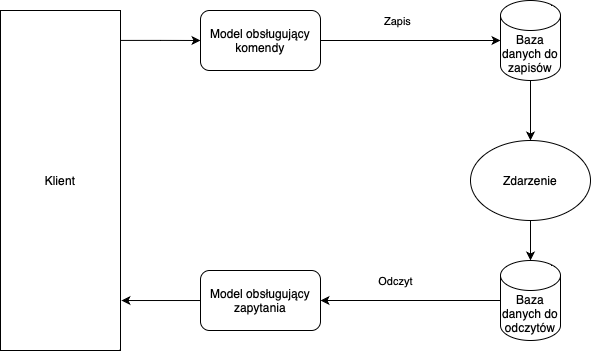
\includegraphics[width=0.6\linewidth]{cqrs.png}
    \caption{Schemat architektoniczny implementacji wzorca CQRS}
\end{figure}

\subsection{Event Sourcing}

Wzorzec Event Sourcing jest podejściem w projektowaniu oprogramowania, które polega na przechowywaniu zmian stanu aplikacji jako sekwencji zdarzeń. Każda akcja w systemie generuje zdarzenie, które zamiast modyfikować stan bezpośrednio, jest rejestrowane i służy jako podstawa do odtworzenia bieżącego stanu systemu.

\begin{enumerate}

    \item Śledzenie Zmian Stanu: Event Sourcing umożliwia śledzenie wszystkich zmian stanu systemu poprzez zapisywanie każdego zdarzenia. To podejście zapewnia kompletną historię zmian, co jest szczególnie przydatne w przypadkach wymagających audytu lub debugowania.

    \item Odtwarzanie Stanu: W Event Sourcing stan aplikacji można odtworzyć poprzez przetworzenie sekwencji zdarzeń. Ta zdolność do "odtworzenia przeszłości" jest bardzo cenna w przypadku awarii lub potrzeby analizy historycznych danych, np. podejrzenie stanu systemu na konkretny dzień.

    \item Integracja z CQRS: Event Sourcing często jest stosowany razem z CQRS (Command Query Responsibility Segregation). CQRS oddziela operacje odczytu od zapisu, co w połączeniu z Event Sourcingiem tworzy wydajny i skalowalny model do zarządzania danymi.

    \item Złożoność Implementacji: Jednym z wyzwań stosowania Event Sourcing jest jego złożoność implementacyjna. Wymaga to dokładnego projektowania systemu i może prowadzić do zwiększenia złożoności kodu, szczególnie w przypadku systemów o dużej skali.

    \item Zarządzanie Zdarzeniami: Event Sourcing wymaga skutecznego zarządzania i przetwarzania strumieni zdarzeń, co może być wyzwaniem w dużych systemach. Ważne jest zapewnienie odpowiedniej wydajności i skalowalności mechanizmów przetwarzających zdarzenia, tzw. magazynu zdarzeń i kolejki komunikatów.

    \item Odzyskiwanie i Odporność na Awarii: Wzorzec ten zapewnia naturalną odporność na awarie, ponieważ stan aplikacji może być odtworzony z historii zdarzeń. Jest to szczególnie ważne w środowisku rozproszonym, jakim jest architektura mikroserwisowa.

    \item Wersjonowanie Zdarzeń: W miarę rozwoju systemu, format zdarzeń może się zmieniać. Zarządzanie różnymi wersjami zdarzeń i ich kompatybilnością wsteczną staje się istotnym aspektem projektu.

\end{enumerate}

\begin{figure}[!h]
    \centering 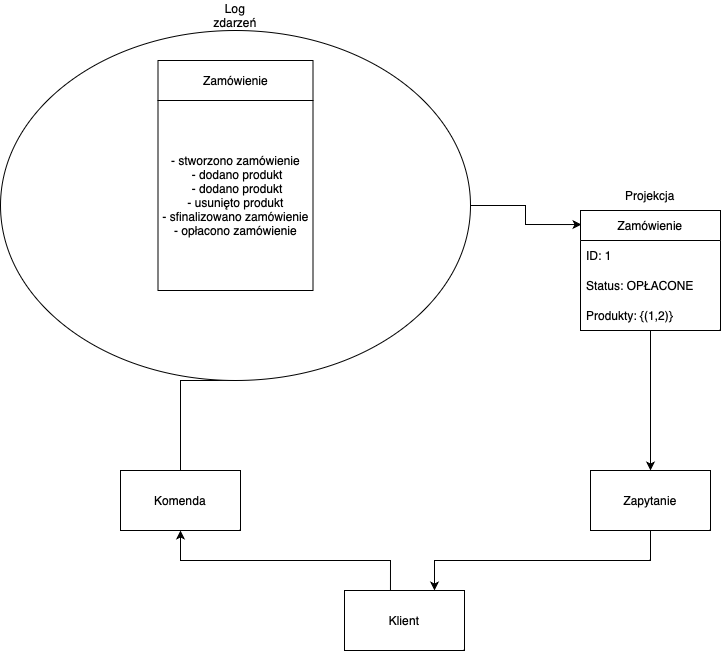
\includegraphics[width=0.6\linewidth]{event_sourcing.png}
    \caption{Schemat architektoniczny implementacji wzorca Event Sourcing}
\end{figure}

\subsection{Wzorzec Saga}

Wzorzec Saga w architekturze mikroserwisowej jest strategią zarządzania transakcjami rozproszonymi. W systemach opartych na mikroserwisach, gdzie każdy serwis zarządza własną bazą danych, tradycyjne transakcje bazodanowe (jak te stosowane w monolitycznych architekturach) nie są możliwe. Saga oferuje rozwiązanie tego problemu, umożliwiając realizację operacji, które obejmują wiele serwisów, poprzez sekwencję lokalnych transakcji.

\begin{enumerate}

    \item Definicja Sag: Saga to sekwencja operacji, w której każda operacja jest lokalną transakcją w ramach jednego mikroserwisu. Jeśli wszystkie operacje zakończą się pomyślnie, cała Saga jest uznawana za zakończoną sukcesem. Jeśli jednak jedna z operacji zawiedzie, Saga inicjuje serię kompensacyjnych akcji, aby przywrócić system do spójnego stanu.

    \item Orkiestracja vs Choreografia: Istnieją dwa podejścia do implementacji Sag: orkiestracja i choreografia. W orkiestracji, centralny koordynator (taki jak serwis orkiestracyjny) zarządza kolejnością i rezultatem operacji. W choreografii, każdy mikroserwis zna kolejny krok i samodzielnie publikuje zdarzenia, które są słuchane przez inne serwisy.

    \item Kompensacja: Gdy jedna z operacji w Sadze zawodzi, system musi podjąć akcje kompensacyjne, aby cofnąć zmiany wprowadzone przez poprzednie operacje. Wymaga to starannego projektowania logiki kompensacji dla każdej operacji.

\end{enumerate}

TODO jakiś rysunek lub snippet?    % Umożliwia to również łatwą migrację do nowej wersji szablonu:
\clearpage % Rozdziały zaczynamy od nowej strony.

\section{Analiza wymagań systemu}

Przed rozpoczęciem implementacji systemu należy go przeanalizować pod kątem wymagań funkcjonalnych oraz niefunkcjonalnych. Twórca powinien uprzednio poznać występujące rodzaje danych, udostępniane na nich operacje oraz klasy użytkowników.

W systemach o architekturze mikroserwisowej należy również odpowiednio wydzielić serwisy, stanowiące spójną całość.

W tym rozdziale zostaną też przedstawione najważniejsze terminy i pojęcia używane w aplikacji, jej wymagania oraz przypadki użycia.

\subsection{Słownik dziedziny problemu}

Słownik najważniejszych pojęć występujących w dziedzinie systemu. W nawiasach podano ich angielskie odpowiedniki, ponieważ w takiej formie zostały one użyte w kodzie aplikacji.

\begin{itemize}

    \item \textbf{Użytkownik zamawiający} (ang. \textit{Ordering User}) - encja reprezentująca użytkownika systemu, odpowiedzialnego za składanie zamówień. Użytkownik taki może definiować swoje adresy dostawy, oraz posiadać historię zamówień. Jest on definiowany przez nazwę oraz adres e-mail.
    \item \textbf{Restauracja} (ang. \textit{Restaurant}) - encja reprezentująca restaurację, która może być obsługiwana przez system. Restauracja posiada menu, które może być modyfikowane przez managera restauracji. Restauracja może być otwarta lub zamknięta, a jej manager może przyjmować lub odrzucać zamówienia. Restauracja jest definiowana przez nazwę, adres, menu oraz managera.
    \item \textbf{Kurier} (ang. \textit{Courier}) - encja reprezentująca dostawcę, który może być przypisany do zamówienia. Kurier może być dostępny lub niedostępny, a jego status może być aktualizowany samodzielne. Posiada on również lokalizację w postaci współrzędnych geograficznych. Kurier jest definiowany przez nazwę, adres e-mail oraz status.
    \item \textbf{Dostawa} (ang. \textit{Order Delivery}) - encja reprezentująca dostawę zamówienia przez kuriera z restauracji do użytkownika. Dostawa posiada status, który może być aktualizowany przez system. Dostawa jest definiowana przez zamówienie, kuriera, lokalizację restauracji, lokalizację użytkownika, obliczoną opłatę dla kuriera oraz status.
    \item \textbf{Zamówienie} (ang. \textit{Order}) - encja reprezentująca zamówienie użytkownika. Zamówienie posiada status, który może być aktualizowany przez system. Zamówienie jest definiowane przez użytkownika, restaurację, adres dostawy, listę dań oraz status.
    \item \textbf{Faktura} (ang. \textit{Invoice}) - encja reprezentująca fakturę wystawioną przez system. Faktura może być wystawiona dla użytkownika, restauracji lub kuriera. Faktura jest definiowana przez składniki, kwotę, datę wystawienia oraz adres e-mail odbiorcy.
    \item \textbf{Płatność} (ang. \textit{Order Payment}) - encja reprezentująca płatność za zamówienie. Płatność może być dokonana przez użytkownika. Płatność jest definiowana przez zamówienie, metodę płatności, kwotę oraz status.
    \item \textbf{Odbiora płatności} (ang. \textit{Payee}) - encja reprezentująca odbiorcę płatności. Odbiorca płatności może być restauracją lub kurierem. Odbiorca płatności jest definiowany przez nazwę, adres e-mail oraz balans kwotowy.
    \item \textbf{Płatnik} (ang. \textit{Payer}) - encja reprezentująca płatnika. Płatnik może być użytkownikiem lub systemem. Płatnik jest definiowany przez nazwę oraz adres e-mail.
    \item \textbf{Zamówienie restauracyjne} (ang. \textit{Restaurant Order}) - encja reprezentująca zamówienie złożone w restauracji. Zamówienie restauracyjne posiada status, który może być aktualizowany przez system. Zamówienie restauracyjne jest definiowane przez restaurację, listę dań oraz status.

\end{itemize}

\subsection{Burza Zdarzeń}

Aby móc podzielić system informatyczny na komponenty, później przekształcone w mikroserwisy, można zastosować np. technikę Burzy Zdarzeń (ang. Event Storming).

Burza Zdarzeń to metoda warsztatowa używana w projektowaniu i analizie systemów opartych na mikroserwisach. Została opracowana przez Alberto Brandoliniego i polega na interaktywnym modelowaniu procesów biznesowych poprzez identyfikację i dyskusję na temat "zdarzeń" mających znaczenie biznesowe. Uczestnicy, wykorzystując kolorowe karteczki, reprezentują różne aspekty systemu, takie jak wydarzenia, komendy, czy modele danych. Ta metoda sprzyja współpracy między różnymi zespołami, pomagając im lepiej zrozumieć procesy biznesowe i technologiczne oraz identyfikować potencjalne problemy i możliwości dla architektury mikroserwisowej.

\begin{figure}[!h]
    \centering 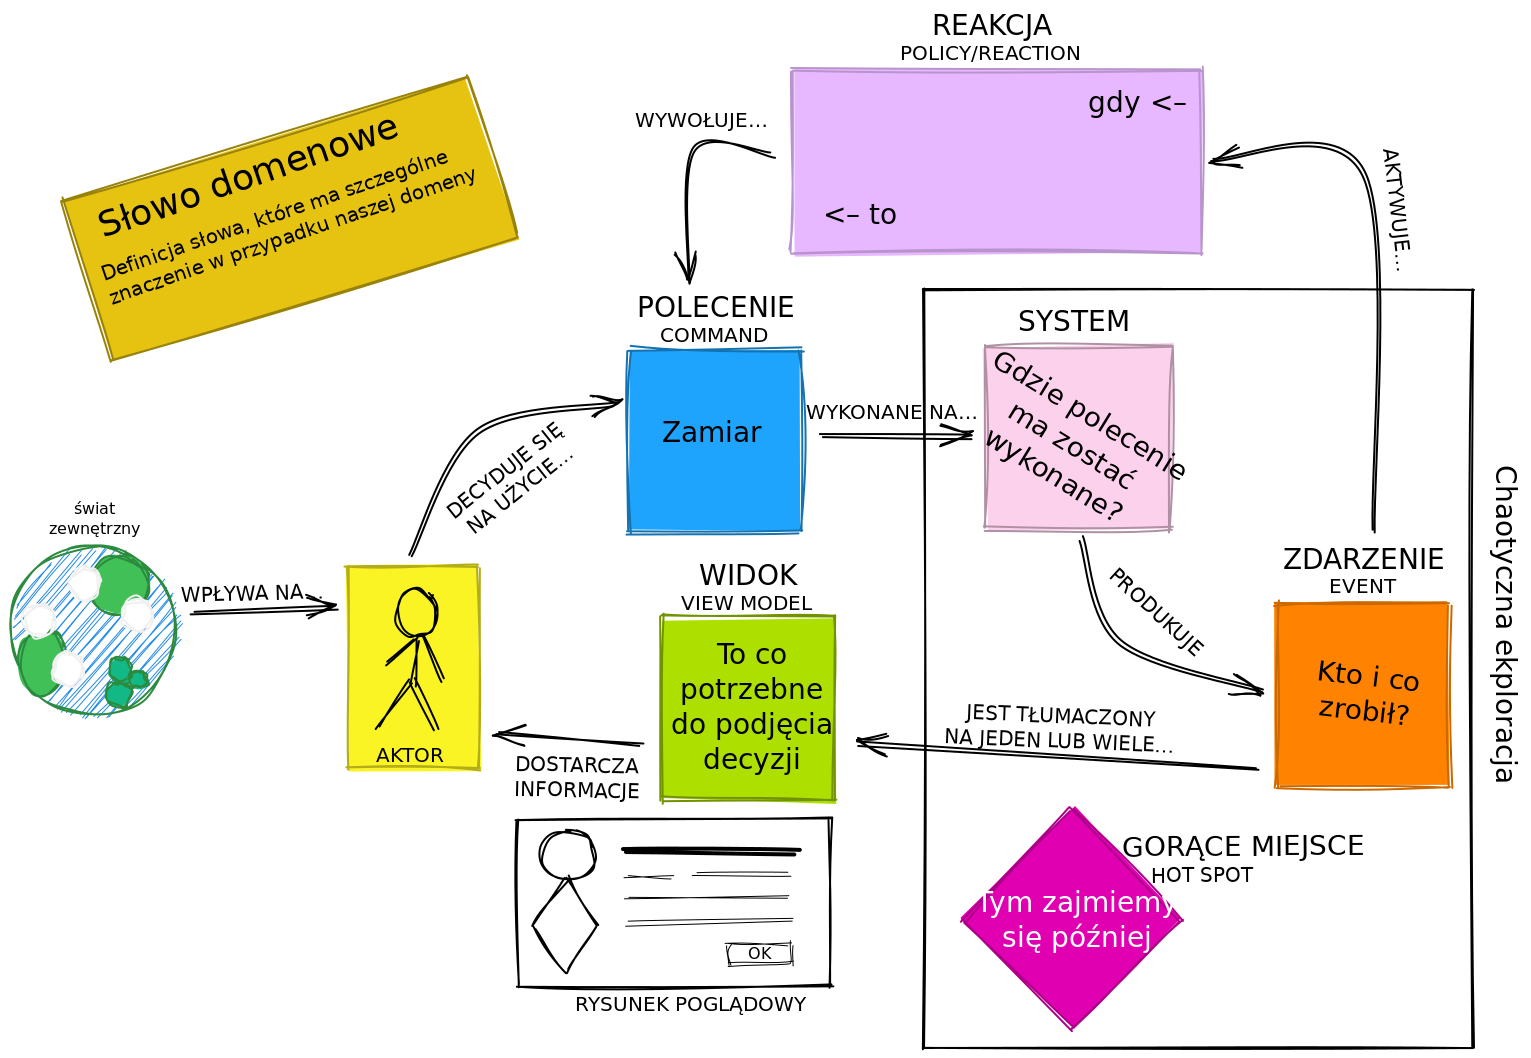
\includegraphics[width=0.8\linewidth]{event_storming.png}
    \caption{Przykładowy rezultat sesji Burzy Zdarzeń \cite{event_storming_rys}}
\end{figure}


Rezultatem sesji Burzy Zdarzeń powinna być lista zdarzeń zgrupowanych w ramach tzw. agregatów dziedzinowych, czyli obiektów realizujących konkretny zbiór logiki biznesowej. W tej postaci łatwo postawić granice między słabo powiązanymi grupami agregatów. Zbiór agregatów po jednej stronie granicy nazywamy Ograniczonym Kontekstem (ang. Bounded Context \cite{boundedcontext})). Są to kandydaci do wydzielenia jako mikroserwisy modelowanej aplikacji.

W ramach pracy inżynierskiej przeprowadzono dla projektowanego systemu sampdzielną sesję Burzy Zdarzeń z wykorzystaniem narzędzia Miro.

Miro \cite{miro} to interaktywna platforma webowa, umożliwiająca tworzenie tablic z notatkami, rysunkami i diagramami. Wybór tego narzędzia był podyktowany jego prostotą użytkowania oraz możliwościami wizualizacji efektów.

W ramach sesji przeprowadzono kolejno następujące kroki:

\begin{itemize}

    \item \textbf{Definicja zdarzeń biznesowych}: Zidentyfikowano kluczowe zdarzenia w procesie biznesowym i zapisuno je na karteczkach (np. "zamówienie złożone", "płatność przyjęta").
    \item \textbf{Układanie zdarzeń}: Zdarzenia zostały ułożone w kolejności chronologicznej, tworząc w ten sposób proces biznesowy.
    \item \textbf{Identyfikacja komend}: Zidentyfikowano komendy, które mogą wywołać zdarzenia (np. "złóż zamówienie").
    \item \textbf{Identyfikacja modeli}: Zidentyfikowano modele danych, które są potrzebne do realizacji procesu biznesowego (np. "zamówienie").
    \item \textbf{Identyfikacja agregatów}: Zidentyfikowano agregaty dziedzinowe, czyli grupy powiązanych ze sobą zdarzeń, komend i modeli danych (np. "zamówienie").
    \item \textbf{Identyfikacja ograniczonych kontekstów}: Zidentyfikowano ograniczone konteksty, czyli grupy powiązanych ze sobą agregatów dziedzinowych (np. "zamówienie").
    \item \textbf{Identyfikacja widoków}: Zidentyfikowano widoki, czyli dane, które są potrzebne do wyświetlenia w interfejsie użytkownika (np. "lista restauracji").

\end{itemize}

\begin{figure}[!h]
    \centering 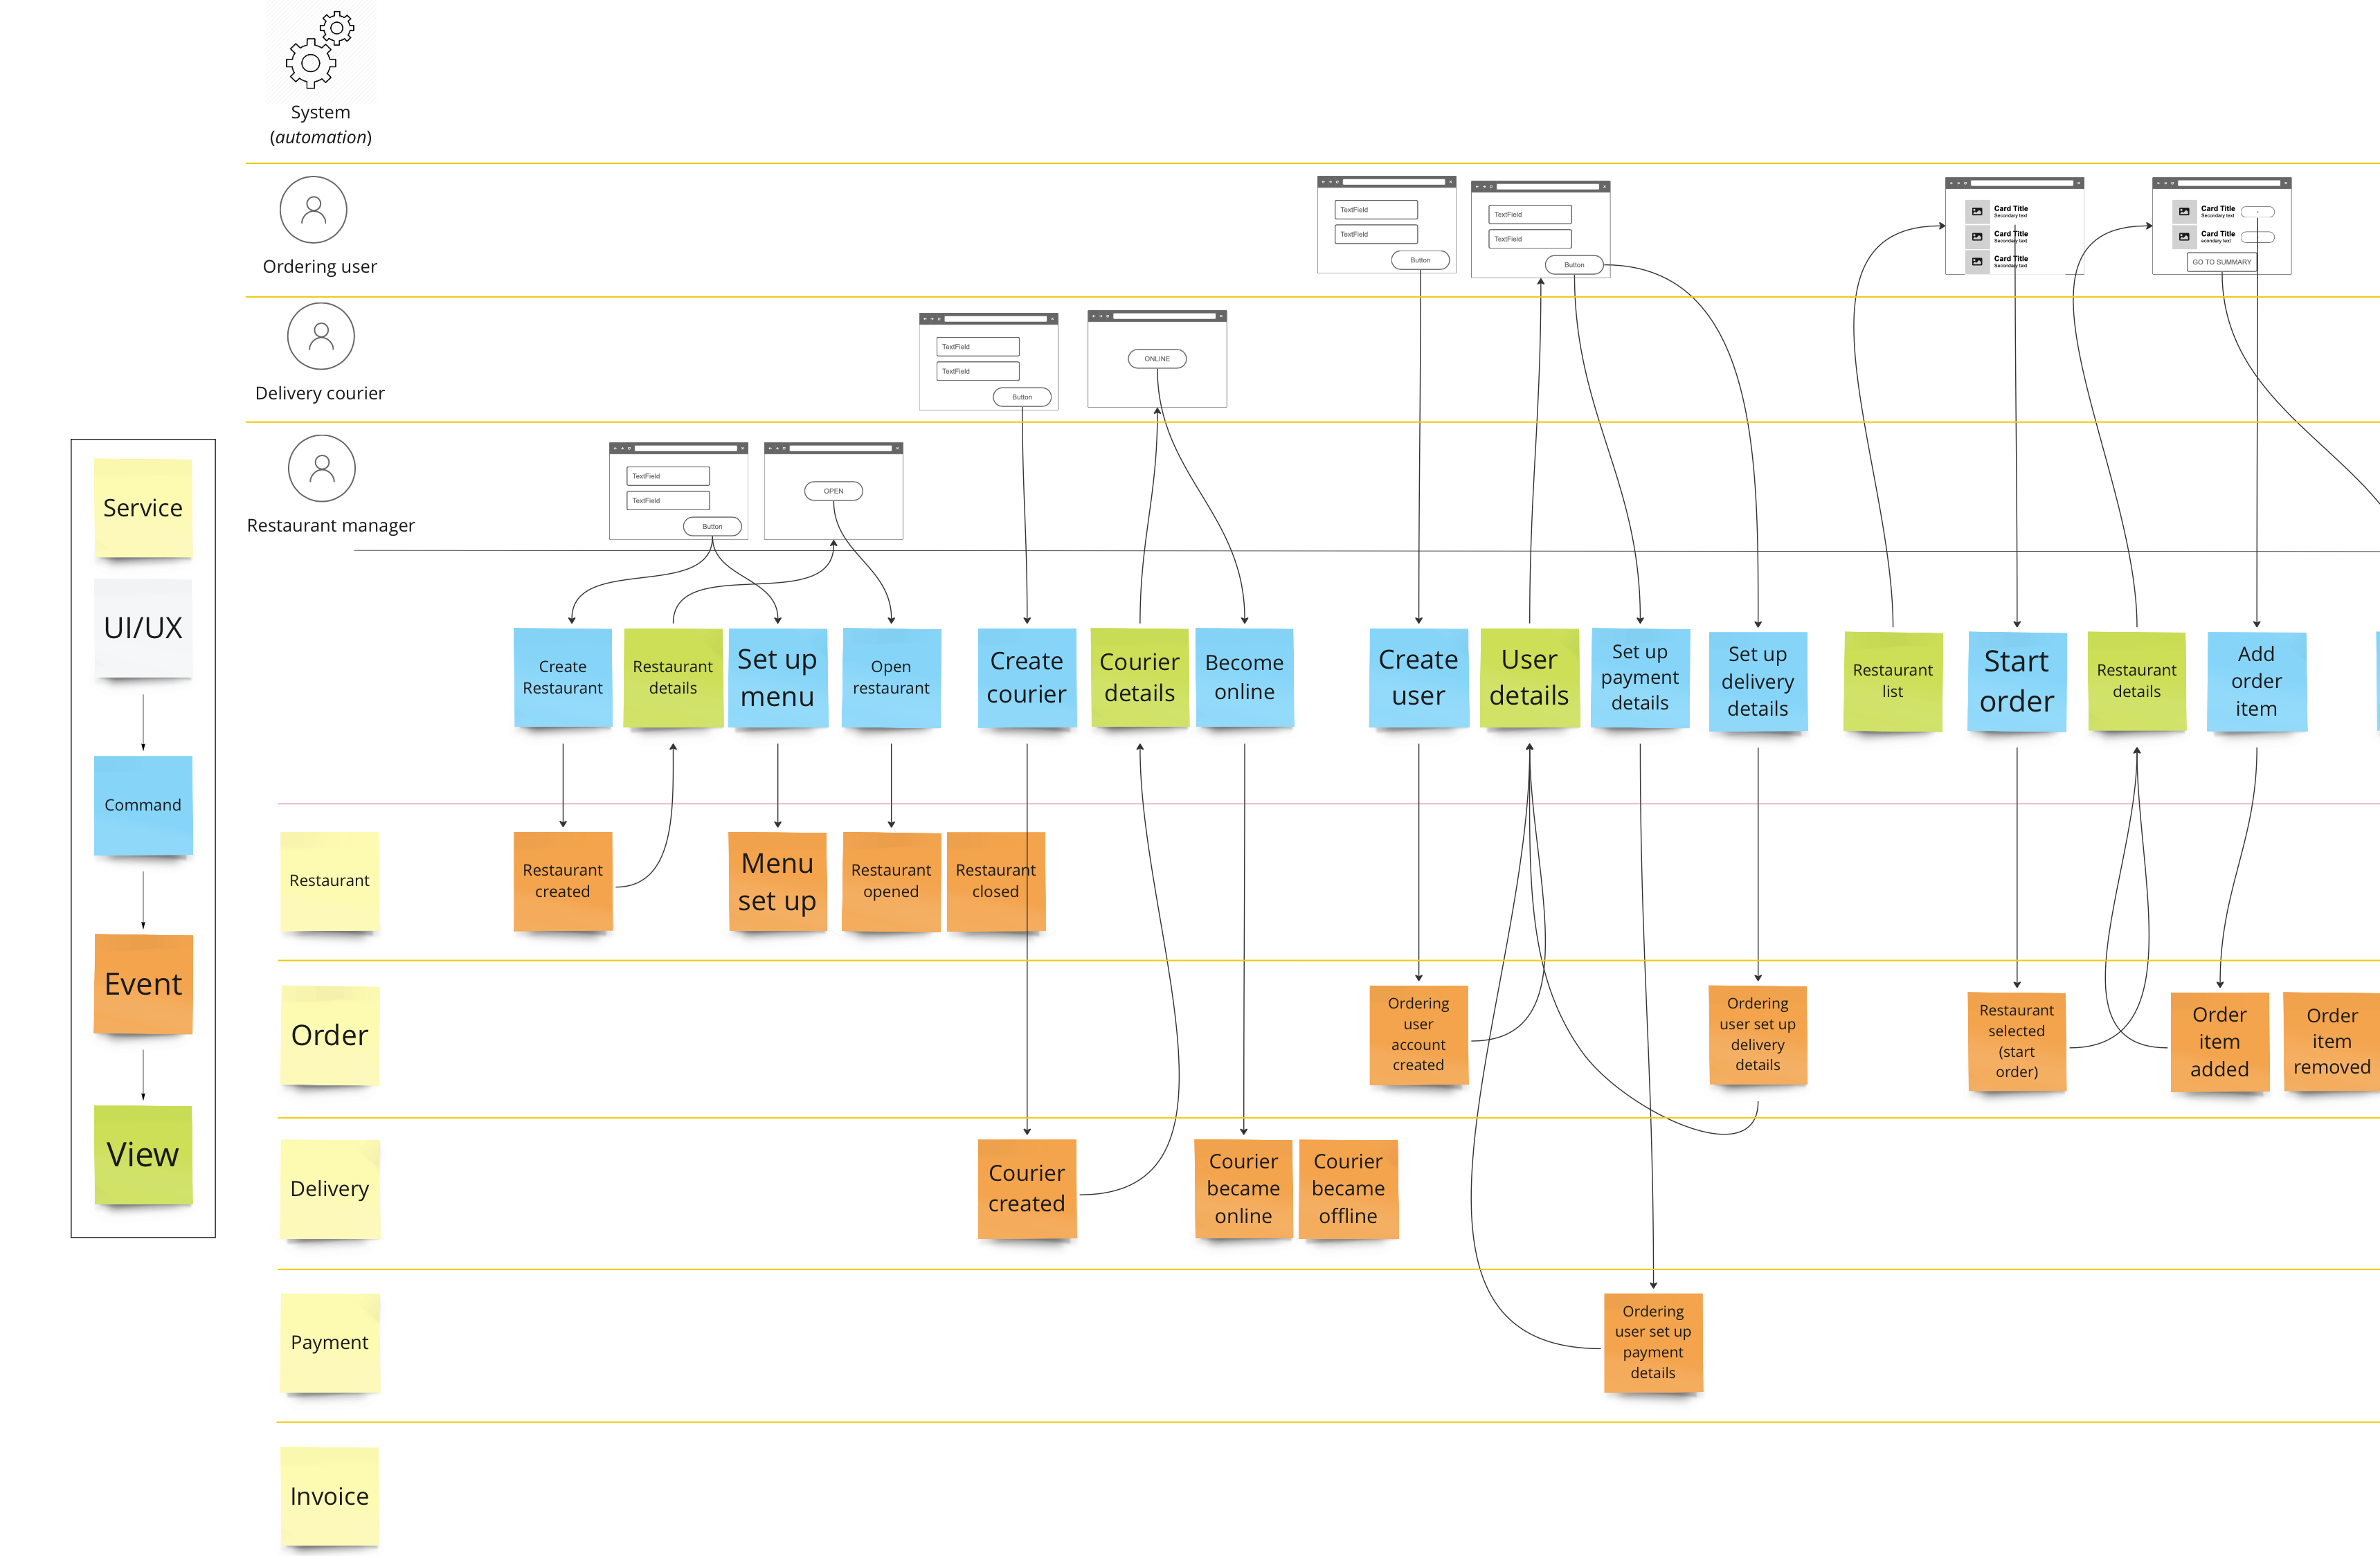
\includegraphics[width=0.8\linewidth]{event_storming2.png}
    \caption{Rezultat sesji Burzy Zdarzeń dla projektowanego systemu}
\end{figure}

\subsection{Identyfikacja Ograniczonych Kontekstów}

W wyniku sesji Burzy Zdarzeń zidentyfikowano pięć kontekstów granicznych, które będą kluczowe dla tworzonej aplikacji. Są to:

\textbf{Restaurant} (\textit{Restauracja}) - obejmuje zarządzanie restauracjami, menu oraz definicją i dostępnością produktów. Potrafi wyliczyć aktualną cenę produktów w zamówieniu oraz zwalidować ich dostępność,

\textbf{Order} (\textit{Zamówienie}) - odpowiada za proces zamówienia, jego składanie, modyfikowanie, anulowanie oraz koordynuje cały proces przygotowania zamówienia do momentu dostawy. Umożliwia również zarządzanie danymi użytkowników i ich adresami dostaw,

\textbf{Delivery} (\textit{Dostawa}) - koncentruje się na logistyce dostaw, monitorowaniu statusu dostawy oraz komunikacji z dostawcą. Zarządza również bazą dostawców i ich lokalizacjami. Odpowiada za proces dopasowania dostawcy do zamówienia,

\textbf{Payment} (\textit{Płatność}) - zarządza procesem płatności, obejmuje różne metody płatności oraz obsługę transakcji. Obsługuje wszelkie rozliczenia w ramach systemu. Odpowiada również za generowanie faktur dla użytkowników, restauracji i dostawców i ich wysyłkę,

\medskip

Powyższe cztery konteksty stały się podstawą do wydzielenia mikroserwisów w ramach projektowanego systemu. Każdy z nich będzie realizowany przez osobny komponent.

\subsection{Wymagania funkcjonalne}

Wymagania funkcjonalne zostały zidentyfikowane na podstawie komend i zdarzeń, które zostały wylistowane w ramach sesji Burzy Zdarzeń. Są to, z podziałem na klasy użytkowników:

\medskip

\textbf{Jako użytkownik zamawiający}
\begin{itemize}
    \item mogę utworzyć konto w systemie,
    \item mogę uwierzytelnić się przy pomocy loginu i hasła lub konta Google,
    \item mogę dodać detale dostawy,
    \item mogę wylistować restauracje wraz z ich średnią oceną,
    \item mogę rozpocząć proces zamówienia wybierając restaurację,
    \item mogę wybrać dania z menu i dodać je do zamówienia,
    \item mogę złożyć zamówienie,
    \item mogę opłacić zamówienie przy użyciu zewnętrznej bramki płatności,
    \item mogę śledzić status zamówienia,
    \item mogę wylistować historyczne zamówienia,
    \item mogę otrzymać fakturę za zamówienie na podany adres e-mail.
\end{itemize}

\medskip

\textbf{Jako manager restauracji}
\begin{itemize}
    \item mogę utworzyć konto restauracji w systemie,
    \item mogę uwierzytelnić się przy pomocy loginu i hasła lub konta Google,
    \item mogę zaktualizować detale i dostępność (otwarta/zamknięta) restauracji,
    \item mogę skonfigurować menu restauracji,
    \item mogę wylistować zamówienia będące w trakcie,
    \item mogę wylistować zamówienia historyczne,
    \item mogę przyjąć zamówienie do realizacji,
    \item mogę odrzucić zamówienie,
    \item mogę oznaczyć zamówienie jako gotowe,
    \item mogę wypłacić środki za zamówienia na podany numer konta,
    \item mogę otrzymać fakturę za zamówienie na podany adres e-mail.
\end{itemize}

\medskip

\textbf{Jako dostawca}
\begin{itemize}
    \item mogę utworzyć konto w systemie,
    \item mogę uwierzytelnić się przy pomocy loginu i hasła lub konta Google,
    \item mogę zaktualizować swój status (dostępny/niedostępny),
    \item mogę zobaczyć dostępną ofertę dostawy,
    \item mogę przyjąć albo odrzucić ofertę dostawy,
    \item mogę zaktualizować status dostawy (odebrana z restauracji, dostarczona do użytkownika),
    \item mogę wylistować historyczne dostawy,
    \item mogę wypłacić środki za dostarczone zamówienia na podany numer konta,
    \item mogę otrzymać fakturę za dostarczone zamówienia na podany adres e-mail.
\end{itemize}

\subsection{Przypadki użycia}

TODO

\subsection{Wymagania niefunkcjonalne}

Wymagania niefunkcjonalne zostały zidentyfikowane m.in. na podstawie ograniczeń biznesowych, wymagań funkcjonalnych oraz doświadczenia Autora w budowaniu skalowalnych aplikacji webowych. Ponadto zostały one zainspirowane listą 12 czynników wpływających na jakość oprogramowania zaproponowaną przez Adama Wigginsa \cite{12factors}.

\textbf{Skalowalność} - każdy z komponentów systemu powinien być skalowalny poziomo w zależności od obciążenia. Każdy mikroserwis powinien móc być replikowalny,

\textbf{Wydajność} - system powinien umożliwiać równoległe przetwarzanie minimum 50 dowolnych żądań HTTP na sekundę,

\textbf{Wysoka dostępność} - możliwość częściowej pracy pomimo utraty niektórych komponentów systemu. System powinien być odporny na awarie,

\textbf{Monitorowanie} - aplikacja powinna umożliwiać monitorowanie i logowanie zdarzeń w celu analizy i debugowania. Każdy mikroserwis powinien logować swoje zdarzenia w centralnym repozytorium, a system powinien umożliwiać monitorowanie stanu mikroserwisów.

\textbf{Testowalność} - system powinien być łatwy do testowania, zarówno jednostkowo jak i integracyjnie oraz wydajnościowo.

\textbf{Bezpieczeństwo} - aplikacja powinna zapewniać odpowiednie zabezpieczenia w celu ochrony poufności, integralności i dostępności danych. Dostęp do mikroserwisów powinien być chroniony przez autoryzację i uwierzytelnianie, a dane powinny być szyfrowane w tranzycie.

\textbf{Synchronizacja i spójność danych} - system powinien zapewniać ostateczną spójność danych pomiędzy mikroserwisami.
\clearpage % Rozdziały zaczynamy od nowej strony.

\section{Architektura systemu}

Potrzebna taka osobna sekcja?

\subsection{Podział na mikroserwisy}

XXX

\subsection{Model C4 systemu}

XXX

\subsection{Persystencja danych}

XXX

\subsection{Kolejka komunikatów i magazyn zdarzeń}

XXX

\subsection{Uwierzytelnianie i autoryzacja}

XXX

\subsection{Integracje zewnętrzne}

XXX
\clearpage % Rozdziały zaczynamy od nowej strony.

\section{Implementacja}

Rozdział ten ma na celu szczegółowy opis implementacji systemu. Zostaną w nim przedstawione wykorzystane narzędzia, podział na moduły oraz szczegóły implementacyjne. Swoje miejsce znajdą tutaj również fragmenty kodu źródłowego, które mają na celu ułatwić zrozumienie sposobu działania systemu.

\subsection{Część serwerowa}

Część serwerową systemu stanowi aplikacja o architekturze mikroserwisowej, napisana w języku Kotlin z wykorzystaniem frameworków Spring Boot oraz Axon Framework.

\subsubsection{Użyte narzędzia}

W części serwerowej aplikacji wykorzystano następujące najważniejsze narzędzia:

\textbf{Kotlin} \cite{kotlin} to język programowania stworzony przez firmę JetBrains, działający na maszynie wirtualnej Javy (JVM) \cite{jvm}. Kotlin jest językiem statycznie typowanym, który łączy w sobie cechy zarówno języków obiektowych, jak i funkcyjnych. Jest on kompilowany do kodu bajtowego Javy, a jego składnia jest w dużej mierze zgodna z Javą, co czyni go łatwym do nauki i zrozumienia dla programistów Javy. Kotlin jest językiem wieloplatformowym, co oznacza, że może być kompilowany do kodu bajtowego Javy, kodu bajtowego Javy na Androida, kodu JavaScript oraz kodu natywnego. Kotlin jest językiem ogólnego przeznaczenia, który może być wykorzystywany do tworzenia aplikacji webowych, mobilnych, desktopowych, a nawet do tworzenia skryptów. Jego jedną z ważniejszych zalet jest wprowadzenie nullowalności na poziomie systemu typów, co pozwala na wykrywanie błędów związanych z niepoprawnym użyciem wartości null w czasie kompilacji, a nie w czasie działania programu.

\textbf{Spring Boot} \cite{springboot} to framework w ekosystemie Spring, który ułatwia tworzenie i rozwijanie aplikacji webowych oraz mikroserwisów w językach Java i Kotlin. Spring Boot oferuje wsparcie dla mikroserwisów, ułatwiając ich tworzenie, testowanie i wdrażanie, co czyni go popularnym wyborem wśród programistów pracujących nad nowoczesnymi, skalowalnymi aplikacjami.

Spring Boot ma silne powiązanie z koncepcją "cloud native", która odnosi się do projektowania aplikacji specjalnie na potrzeby chmury. Spring Boot ułatwia tworzenie aplikacji mikroserwisowych, które są nieodzownym elementem architektury cloud native, dostarczając funkcjonalności takie jak łatwa integracja z kontenerami (np. Docker), obsługa konfiguracji zewnętrznej, zarządzanie usługami przez service discovery oraz wspieranie wzorców takich jak circuit breaker. Te cechy sprawiają, że Spring Boot jest idealnym wyborem dla tworzenia aplikacji przygotowanych do działania w środowiskach chmurowych, oferujących skalowalność, elastyczność i odporność.

\textbf{Axon Framework} to framework do tworzenia aplikacji w architekturze opartej na zdarzeniach (event-driven) i wzorcu CQRS. Wspiera również DDD, Event Sourcing oraz wzorzec Saga. Axon Framework jest napisany w języku Java, ale może być wykorzystywany również w języku Kotlin. Axon Framework dostarcza abstrakcje do tworzenia aplikacji opartych na zdarzeniach, takich jak agregaty, komendy, zdarzenia, szyna wiadomości, sagi, itp. Axon Framework jest narzędziem open source, rozwijanym przez firmę AxonIQ.

\textbf{Axon Server} jest infrastrukturalnym elementem ekosystemu Axon, pełniącym rolę kolejki komunikatów oraz magazynu zdarzeń. Oferuje on również narzędzia do monitoringu i zarządzania aplikacjami opartymi na Axon Framework.

\subsubsection{Architektura heksagonalna}

Część serwerowa aplikacji została zaimplementowana zgodnie z architekturą heksagonalną (ang. hexagonal architecture), która jest jedną z popularnych architektur aplikacji serwerowych, wykorzystywanych przy złożonych projektach informatycznych. Architektura ta jest również znana pod nazwą architektury czystej (ang. clean architecture) lub architektury portów i adapterów (ang. ports and adapters architecture). Została ona zaproponowana przez Alistaira Cockburna w 2005 roku \cite{cockburn2005hexagonal}.

Architektura heksagonalna jest architekturą warstwową, która składa się z trzech warstw: warstwy adapterów, warstwy dziedziny oraz warstwy infrastruktury. Warstwa dziedziny jest główną warstwą aplikacji, która zawiera logikę biznesową. Warstwa adapterów jest warstwą zewnętrzną, która zawiera adaptery wejściowe i wyjściowe, które są odpowiedzialne za komunikację z zewnętrznymi systemami. Warstwa infrastruktury jest warstwą wewnętrzną, która zawiera implementację adapterów wejściowych i wyjściowych. Warstwa infrastruktury jest odpowiedzialna za konfigurację aplikacji oraz za integrację z zewnętrznymi systemami (np. bazą danych, systemem plików, itp.).

\subsubsection{Podział na pakiety}

Z powodu zastosowania architektury heksagonalnej, część serwerowa aplikacji została podzielona na pakiety zgodnie z warstwami tejże architektury. Podział na pakiety przykładowego serwisu został przedstawiony na wycinku \ref{lst:server-packages}.

\begin{lstlisting}[caption={Podział na pakiety części serwerowej projektu},label={lst:server-packages},captionpos=b]
- adapter/
    - in/
    - out/
- domain/
    - query/
    - command/
- config/
- infrastructure/
- Application.kt
\end{lstlisting}

W kolejnych podrozdziałach zostaną przedstawione szczegóły implementacyjne poszczególnych warstw wraz z ich opisem.

\subsubsection{Warstwa adapterów wejściowych} 

Warstwa ta obejmuje pakiet \textit{adapter.in}. Zawiera ona tzw. adaptery wejściowe, czyli komponenty odpowiedzialne za rozpoczynanie przepływu sterowania w aplikacji. Adaptery wejściowe są odpowiedzialne za obsługę zapytań i komend, które są wysyłane do aplikacji przez użytkowników lub inne systemy. W implementowanym systemie adapterami wejściowymi są kontrolery REST API oraz serwisy nasłuchujące na zdarzenia z kolejki komunikatów.

Na wycinku \ref{lst:server-in-adapter} przedstawiono przykładowy kod kontrolera REST API, który obsługuje zapytanie HTTP POST na ścieżce \textit{/api/v1/orders}. Zapytanie to rozpoczyna zamówienie ze strony użytkownika zamawiającego. W ciele zapytania znajduje się obiekt JSON, który jest mapowany na obiekt klasy \textit{StartOrderRequest}. Obiekt ten jest następnie przekazywany do komponentu \textit{ReactorCommandGateway}, który jest odpowiedzialny za wysłanie komendy \textit{StartOrderCommand} do szyny komend. Komenda ta jest następnie przekazywana do odpowiedniego agregatu dziedzinowego, który jest odpowiedzialny za jej obsługę. Rezultatem synchronicznym obsługi komendy jest nadany identyfikator zamówienia, w postacu UUID, który jest zwracany w odpowiedzi HTTP. 

\begin{lstlisting}[caption={Kod kontrolera REST API obsługującego zapytania dotyczące zamówień},label={lst:server-in-adapter},captionpos=b,language=Kotlin,numbers=left]
@RestController
@RequestMapping("/api/v1/orders")
class OrderController(
    private val reactorCommandGateway: ReactorCommandGateway
) {
    @PostMapping
    @ResponseStatus(HttpStatus.CREATED)
    @PreAuthorize("hasAnyAuthority('${Scopes.ORDER.WRITE}')")
    fun startOrder(
        @RequestBody request: StartOrderRequest,
        exchange: ServerWebExchange
    ): Mono<UuidWrapper> {
        val command = mapToStartOrderCommand(request, exchange)
        val id = reactorCommandGateway.send<UUID>(command)
        return id.map { UuidWrapper(it) }
    }
}
\end{lstlisting}

Kod kontrolera został napisany z wykorzystaniem biblioteki programowania reaktywnego Spring WebFlux, która pozwala na obsługę żądań HTTP w sposób asynchroniczny. Pozwala to na obsługę większej liczby żądań przy użyciu mniejszej liczby wątków, co przekłada się na większą wydajność aplikacji.

Poza kodem obsługującym żądanie HTTP, kontroler zawiera również adnotacje, które definiują uprawnienia wymagane do wykonania żądania. W tym przypadku żądanie wymaga posiadania uprawnień \textit{ORDER.WRITE}, które są zdefiniowane w klasie \textit{Scopes}. Jest to część biblioteki Spring Security, implementującej standard OAuth 2.0.

\subsubsection{Warstwa adapterów wyjściowych} 

Warstwa ta obejmuje pakiet \textit{adapter.out}. Zawiera ona tzw. adaptery wyjściowe, czyli komponenty odpowiedzialne za komunikację z zewnętrznymi systemami. W implementowanym systemie adapterami wyjściowymi są komponenty oferujące dostęp do bazy danych oraz komunikację z zewnętrznymi systemami np. Google Maps Platform.

Na wycinku \ref{lst:server-out-adapter} przedstawiono przykładowy kod komponentu oferującego dostęp do bazy danych. Jest to implementacja (adapter) interfejsu (portu) \textit{OrderDeliveryRepository}, który jest odpowiedzialny za zapisywanie i odczytywanie encji \textit{OrderDeliveryEntity} z bazy danych. Implementacja ta wykorzystuje repozytorium Spring Data, które jest komponentem oferującym dostęp do bazy MongoDB. Repozytorium to jest wstrzykiwane do klasy \textit{DbOrderDeliveryRepository} przy pomocy mechanizmu wstrzykiwania zależności oferowanego przez framework Spring. 

\begin{lstlisting}[caption={Kod implementacji repozytorium dziedzinowego projekcji Zamówienia},label={lst:server-out-adapter},captionpos=b,language=Kotlin,numbers=left]
@Service
class DbOrderDeliveryRepository(
    private val repository: SpringDataOrderDeliveryRepository
) : OrderDeliveryRepository {
    override fun save(delivery: OrderDeliveryEntity) {
        repository.save(delivery).block()
    }

    override fun load(id: UUID): OrderDeliveryEntity? {
        return repository.findById(id).block()
    }

    override fun loadOffers(): List<OrderDeliveryEntity> {
        return repository
            .findAllByStatus(DeliveryStatus.OFFER)
            .collectList().block() ?: listOf()
    }
}
\end{lstlisting}

\subsubsection{Warstwa dziedziny} 

Warstwa ta obejmuje pakiet \textit{domain}. Zawiera ona komponenty, które są odpowiedzialne za logikę biznesową aplikacji. W implementowanym systemie komponentami tymi są agregaty dziedzinowe, komendy, zdarzenia, porty, sagi, encje bazodanowe, klasy wyjątków, zapytania, komponenty budujące projekcje oraz obiekty transferu danych.

Warstwa dziedziny jest podzielona zgodnie ze wzorcem CQRS na część komend oraz część zapytań. Część komend jest zawarta w podpakiecie \textit{command}, a część zapytań w podpakiecie \textit{query}.

Na wycinku \ref{lst:server-domain} przedstawiono częściowy kod komponentów warstwy dziedziny odpowiadającej za rozpoczynanie zamówienia z perspektywy użytkownika systemu. Są to: agregat dziedzinowy \textit{Order}, komenda \textit{StartOrderCommand} oraz zdarzenie \textit{OrderStartedEvent}. Przedstawiono również zawartość portu \textit{OrderVerificationPort}, który jest odpowiedzialny za wstępną walidację zamówienia.

\begin{lstlisting}[caption={Kod komponentów odpowiedzialnych za rozpoczynanie zamówień},label={lst:server-domain},captionpos=b,language=Kotlin,numbers=left]
@Aggregate
internal class Order {

    @AggregateIdentifier
    private lateinit var id: UUID
    private lateinit var status: OrderStatus

    @AggregateMember
    private val items: MutableMap<UUID, Int> = mutableMapOf()

    @CommandHandler
    constructor(
        command: StartOrderCommand,
        orderVerificationPort: OrderVerificationPort
    ) {
        require(
            orderVerificationPort.restaurantExists(command.restaurantId)
        )
        require(
            orderVerificationPort.isRestaurantOpen(command.restaurantId)
        )

        apply(
            OrderStartedEvent(
                orderId = command.orderId,
                restaurantId = command.restaurantId,
                userId = command.userId,
                status = OrderStatus.CREATED
            )
        )
    }
}

data class StartOrderCommand(
    @TargetAggregateIdentifier val orderId: UUID,
    val userId: String,
    val restaurantId: UUID
)

data class OrderStartedEvent(
    val orderId: UUID,
    val restaurantId: UUID,
    val userId: String,
    val status: OrderStatus
)

interface OrderVerificationPort {
    fun restaurantExists(restaurantId: UUID): Boolean
    fun isRestaurantOpen(restaurantId: UUID): Boolean
}
\end{lstlisting}

Kod ten jest wywoływany w momencie otrzymania komendy \textit{StartOrderCommand} przez agregat \textit{Order}. Komenda ta jest wysyłana do agregatu przez adapter wejściowy, zaprezentowany w rozdziale 5.1.4. Agregat \textit{Order} jest odpowiedzialny za wstępną walidację zamówienia, która jest realizowana przy pomocy portu \textit{OrderVerificationPort}. W przypadku tej komendy, system weryfikuje czy podana resutacja istnieje i czy jest otwarta. Port walidacyjny jest interfejsem, implementowanym przez odpowiedni adapter wyjściowy.

W przypadku, gdy wstępna walidacja zamówienia zakończy się sukcesem, agregat \textit{Order} emituje zdarzenie \textit{OrderStartedEvent}, które jest zapisywane w magazynie zdarzeń, kontrolowanym przez Axon Server. Na zdarzenie nasłuchują inne komponenty systemu, które mogą na jego podstawie budować projekcje, wysyłać powiadomienia do użytkowników, lub podejmować inne akcje.

Dzięki zastosowaniu Axon Framework nie ma konieczności pisania kodu odpowiedzialnego za ładowanie agregatów dziedzinowych, wywoływanie odpowiednich metod obsługujących komendy czy publikowanie zdarzeń. Większość interakcji odbywa się bez udziału programisty, przy pomocy odpowiednich adnotacji, takich jak np. \textit{@Aggregate}, \textit{@AggregateIdentifier}, \textit{@CommandHandler} itp.

\subsubsection{Warstwa prezentacji/zapytań}

Warstwa ta obejmuje pakiet \textit{query}. Zawiera ona komponenty, które są odpowiedzialne za obsługę zapytań użytkowników systemu. W implementowanym systemie komponentami tymi są procesory zdarzeń budujące projekcje, zapytania oraz klasy pomocnicze służące do persystencji danych w bazie danych.

Na wycinku \ref{lst:server-domain-query} przedstawiono kod procesora zdarzeń budującego projekcję zamówienia. Procesor ten nasłuchuje na zdarzenie \textit{OrderStartedEvent} i na jego podstawie buduje projekcję zamówienia, która jest zapisywana w bazie danych. Procesor ten jest wywoływany automatycznie przez Axon Framework, w momencie otrzymania odpowiednigo zdarzenia.

\begin{lstlisting}[caption={Kod procesora zdarzeń budującego projekcję zamówienia},label={lst:server-domain-query},captionpos=b,language=Kotlin,numbers=left,showstringspaces=false]
@ProcessingGroup("projection")
class OrderHandler(
    private val orderRepository: OrderRepository,
    private val restaurantRepository: RestaurantRepository
) {

    @EventHandler
    fun on(event: OrderStartedEvent) {
        val restaurant = restaurantRepository.load(
            event.restaurantId
        )

        val restaurantLocation = restaurant?.location 
            ?: error("Restaurant not found")

        val entity = OrderEntity(
            id = event.orderId,
            restaurantId = event.restaurantId,
            restaurantLocation = restaurantLocation,
            userId = event.userId,
            status = OrderStatus.CREATED,
            items = mutableMapOf(),
            createdAt = Instant.now()
        )
        orderRepository.save(entity)
    }
}
\end{lstlisting}

\subsubsection{Warstwa konfiguracji}

Warstwa ta obejmuje pakiet \textit{config}. Zawiera ona komponenty, które są odpowiedzialne za konfigurację aplikacji.

Przykładowym komponentem w implementowanym systemie jest filtr zapytań, odpowiedzialny za odczytywanie atrybutu \textit{subject} z tokenu JWT oraz zapisywanie go w kontekście żądania. Jest to używane m.in. do poprawnej autoryzacji użytkownika w momencie wywoływania komendy (np. dostęp do zasobu ma tylko jego autor). Kod tego komponentu został przedstawiony na wycinku \ref{lst:server-config}.

\begin{lstlisting}[caption={Kod filtra zapytań},label={lst:server-config},captionpos=b,language=Kotlin,numbers=left,showstringspaces=false]
@Component
@Profile("!nosecurity")
class UserContextWebFilter : WebFilter {
    override fun filter(
        exchange: ServerWebExchange,
        chain: WebFilterChain
    ): Mono<Void> {
        return ReactiveSecurityContextHolder.getContext()
            .mapNotNull { it.authentication.principal }
            .cast(Jwt::class.java)
            .doOnNext {
                val userId = it.subject.removePrefix("auth0|")
                exchange.setUserId(userId)
            }
            .then(chain.filter(exchange))
    }
}
\end{lstlisting}

Dzięki zastosowaniu adnotacji \textit{@Profile("!nosecurity")} możliwe jest wyłączenie tego filtra w trybie \textit{nosecurity}, który jest używany w testach wydajnościowych, w których wyłączone są mechanizmy uwierzytelniania i autoryzacji.

\subsubsection{Warstwa infrastruktury}

Warstwa ta obejmuje pakiet \textit{infrastructure}. Zawiera ona kod, niezwiązany z domeną aplikacji, który jest odpowiedzialny za integrację z konkretnymi technologiami, np. bazą danych, systemem plików, itp. W implementowanym systemie komponentami tej warstwy są np. implementacje repozytoriów bazodanowych używające konkretnej technologii - Spring Data MongoDB. Są to również komponenty służące do komunikacji z zewnętrznymi usługami, np. klient Google Maps Platform.

Na wycinku \ref{lst:server-infrastructure} przedstawiono przykładowy kod implementacji repozytorium bazodanowego. Jest to implementacja interfejsu \textit{ReactiveMongoRepository}, który jest komponentem oferującym dostęp do bazy MongoDB. Mimo faktu, że repozytorium to jest interfejsem, a nie klasą, to dzięki mechanizmowi refleksji oferowanemu przez framework Spring, implementacja ta jest automatycznie generowana w czasie uruchamiania aplikacji.

\begin{lstlisting}[caption={Kod implementacji repozytorium bazodanowego},label={lst:server-infrastructure},captionpos=b,language=Kotlin,numbers=left,showstringspaces=false]
@Repository
interface SpringDataOrderRepository 
    : ReactiveMongoRepository<OrderEntity, UUID> {

    fun findAllByUserId(userId: String): Flux<OrderEntity>
}
\end{lstlisting}

Repozytorium bazowe, \textit{ReactiveMongoRepository} zawiera podstawowe metody do operacji na bazie danych, takie jak np. \textit{save}, \textit{findById}, \textit{findAll}, itp. Repozytorium \textit{SpringDataOrderRepository} rozszerza repozytorium bazowe i dodaje do niego dodatkową metodę \textit{findAllByUserId}, która zwraca wszystkie zamówienia danego użytkownika.

\subsubsection{Współdzielony kod}

Kod współdzielony przez różne serwisy w ramach systemu został umieszczony w osobnym module \textit{shared}. Zawiera on m.in. klasy reprezentujące obiekty transferu danych, wyjątki, stałe, wspólną konfigurację itp.

Moduł ten jest wersjonowany i publikowany jako artefakt systemu budowania Maven, dzięki czemu może być umieszczony w centralnym repozytorium i importowany przez inne projekty.

Przykład współdzielonej klasy zaprezentowany jest na wycinku \ref{lst:server-shared}

\begin{lstlisting}[caption={Kod klasy konfigurującej mechanizm uwierzytelniania i autoryzacji},label={lst:server-shared},captionpos=b,language=Kotlin,numbers=left,showstringspaces=false]
@Configuration
@EnableReactiveMethodSecurity
@EnableWebFluxSecurity
@Profile("!nosecurity")
class SecurityConfig {

    @Bean
    fun springSecurityFilterChain(
        http: ServerHttpSecurity
    ): SecurityWebFilterChain {
        return http.authorizeExchange {
            it.pathMatchers("/actuator/**").permitAll()
            it.pathMatchers("/api/v1/payments/stripe-webhook").permitAll()
            it.anyExchange().authenticated()
        }.csrf {
            it.disable()
        }.cors {
            it.disable()
        }.oauth2ResourceServer {
            it.jwt {}
        }.build()
    }
}
\end{lstlisting}

Klasa ta jest odpowiedzialna za konfigurację mechanizmu uwierzytelniania i autoryzacji. Została ona umieszczona w module \textit{shared}, ponieważ jest ona wspólna dla wszystkich serwisów w ramach systemu. Uruchamia ona mechanizm uwierzytelniania i autoryzacji oferowany przez framework Spring Security. Uwierzytelnianie odbywa się przy pomocy tokenów JWT. Dodatkowo, wyłącza ona mechanizmy obrony przed atakiem CSRF oraz CORS, które są niepotrzebne w przypadku zastosowanej infrastruktury sieciowej systemu.

Domyślnie, żądania na wszystkie ścieżki aplikacji wymagają uwierzytelniania. Są jednak dwie ścieżki, gdzie takie mechanizmy są wyłączone. Pierwsza z nich to ścieżka \textit{/actuator/**}, która jest wykorzystywana przez framework Spring Boot do oferowania statusu aplikacji, wykorzystywanego m.in. przez orkiestratora kontenerów Kubernetes. Druga ścieżka to \textit{/api/v1/payments/stripe-webhook}, która jest wykorzystywana przez serwis odpowiedzialny za płatności, do obsługi webhooków z serwisu Stripe.

\subsection{Część kliencka}

Część kliencka aplikacji została zaimplementowana jako aplikacja przeglądarkowa typu Multi Page Application (MPA) w języku TypeScript z wykorzystaniem frameworków React oraz Remix.

W przeciwieństwie do popularnego obecnie podejścia Single Page Application (SPA), w którym cała aplikacja jest ładowana przy pierwszym wejściu użytkownika na stronę, w podejściu MPA każda strona jest ładowana osobno. MPA wymaga przeładowywania całej strony podczas nawigacji między różnymi widokami, co jest wadą tego podejścia. Zaletą jest jednak to, że każda strona może być ładowana niezależnie, co pozwala na szybsze ładowanie aplikacji, a także na łatwiejsze indeksowanie przez wyszukiwarki internetowe. Upraszcza to również proces tworzenia aplikacji, ponieważ nie ma potrzeby implementowania zaawansowanym mechanizmów trasowania lub zarządzania stanem.

\subsubsection{Użyte narzędzia}

W części klienckiej aplikacji wykorzystano następujące najważniejsze narzędzia:

\textbf{TypeScript} \cite{typescript} to język programowania stworzony przez firmę Microsoft, będący rozszerzeniem języka JavaScript, poprzed wprowadzenie statycznego typowania, co pozwala programistom na wykrywanie błędów w czasie kompilacji i znacząco ułatwia zarządzanie dużymi projektami. 

\textbf{React} \cite{react} to biblioteka JavaScript, która jest wykorzystywana do tworzenia interfejsów użytkownika. React jest deklaratywną biblioteką open source, rozwijaną przez firmę Facebook, która pozwala na tworzenie interfejsów użytkownika przy pomocy komponentów. Może ona być wykorzystywana do tworzenia zarówno aplikacji webowych, jak i mobilnych. W przeciwieństwie do poprzednich podejść w tworzeniu aplikacji internetowych, React stosuje technikę wirtualnego drzewa dokumentu (ang. virtual DOM) do renderowania interfejsu użytkownika. Technika ta polega na przechowywaniu w pamięci drzewa DOM, które jest reprezentacją interfejsu użytkownika. W momencie zmiany stanu aplikacji, drzewo DOM jest aktualizowane, a następnie porównywane z drzewem DOM przechowywanym w pamięci. Na podstawie tego porównania, React aktualizuje tylko te elementy interfejsu użytkownika, które uległy zmianie. Dzięki temu, renderowanie interfejsu użytkownika jest znacznie szybsze, co przekłada się na lepszą wydajność aplikacji.

\textbf{Remix} \cite{remix} to framework do tworzenia aplikacji internetowych typu MPA, oparty na modelu SSR (ang. server side rendering), czyli renderowania interfejsu użytkownika po stronie serwera. Pozwala on na opbieranie danych na poziomie trasowania, co oznacza, że dane są ładowane przed renderowaniem komponentów, co pozwala na szybsze ładowanie aplikacji i lepsze pozycjonowanie w wyszukiwarkach internetowych.

\subsubsection{Podział na katalogi}

Część kliencka aplikacji została podzielona na foldery, grupując w ten sposób różne rodzaje elementów systemu. Podział przedstawiono na wycinku \ref{lst:client-packages}.

\begin{lstlisting}[caption={Podział na foldery części klienckiej projektu},label={lst:client-packages},captionpos=b]
- components/
- routes/
- server/
- services/
- styles/
\end{lstlisting}

W kolejnych podrozdziałach zostaną przedstawione szczegóły implementacyjne poszczególnych warstw wraz z ich opisem.

\subsubsection{Komponenty interfejsu użytkownika}

Komponenty interfejsu użytkownika zostały umieszczone w folderze \textit{components}. Zostały one podzielone na foldery, grupujące komponenty używane w częściach aplikacji przeznaczonych dla różnych klas użytkowników (zamawiających, managerów restauracji i kurierów).

Przykładowy komponent został przedstawiony na wycinku \ref{lst:client-component}. Jest to komponent \textit{Topbar} odpowiedzialny za wyświetlanie paska nawigacji dla managerów restauracji. Przyjmuje on dwa parametry: \textit{payee} oraz \textit{restaurant}. Pierwszy z nich jest obiektem zawierającym informacje o aktualnie zalogowanym użytkowniku, a drugi zawiera informacje o restauracji, w której aktualnie pracuje użytkownik. Komponent ten wyświetla nazwę restauracji oraz jej aktualną dostępność. Dostępność jest wyświetlana w formie przycisku, który po kliknięciu wysyła żądanie HTTP PUT do serwera, w celu zmiany dostępności restauracji.

\begin{lstlisting}[caption={Kod komponentu interfejsu użytkownika - pasek nawigacji managera restauracji},label={lst:client-component},captionpos=b,language=JavaScript,numbers=left,showstringspaces=false]
export default function Topbar(props: TopbarProps) {
    return (
      <header
        className="..."
      >
        <span>Restaurant "{props.restaurant.name}"</span>
        <Form method="post">
          <span className="align-middle inline-block">
            {props.restaurant.availability}
          </span>
          <input
            type="hidden"
            name="availability"
            value={props.restaurant.availability}
          />
          <input
            type="hidden"
            name="restaurantId"
            value={props.restaurant.id}
          />
          <Button 
            type="submit" 
            name="_action" 
            value="update_availability"
          >
            CHANGE
          </Button>
        </Form>
      </header>
    );
}
  
export interface TopbarProps {
  payee: PayeeResponse;
  restaurant: RestaurantResponse;
}
\end{lstlisting}

Odpowiedzialność za dostarczenie danych oraz obsługę formularza komponent ten deleguje do swojego rodzica. Jest to podejście typowe dla biblioteki React, która promuje podejście kompozycyjne do tworzenia interfejsów użytkownika.

\subsubsection{Obsługa ścieżek}

Komponenty aplikacji odpowiedzialne za obsługę ścieżek zostały umieszczone w folderze \textit{routes}. W frameworku Remix, komponenty te są punktami startowymi podróży użytkownika po aplikacji. Na przykład, po podanie w przeglądarce użytkownika ścieżki \textit{/v2/courier/delivery} aplikacja uruchomi plik \textit{courier.delivery.tsx}, który od tego momentu jest odpowiedzialny za ładowanie danych, obsługę formularzy i renderowanie komponentów.

Na wycinku \ref{lst:client-route} przedstawiono kod komponentu obsługującego ścieżkę \textit{/v2/ordering/restaurants} wyświetlającą listę restauracji, które może wybrać użytkownik zamawiający.

\begin{lstlisting}[caption={Kod ścieżki wyświetlającej listę dostępnych restauracji - \textit{/v2/ordering/restaurants}},label={lst:client-route},captionpos=b,language=JavaScript,numbers=left,showstringspaces=false]
export async function loader({ request }: LoaderArgs) {
    const currentUser = await getCurrentUser(request);
    const restaurants = await getRestaurants(request);
  
    const activeOrderId = await getOrderId(request);
    const activeOrder = await getOrder(request, activeOrderId)
  
    return json({ restaurants, currentUser, activeOrder });
}

export async function action({ request, params }: ActionArgs) {
    const formData = await request.formData();
    ...
}

export default function V2RestaurantsPage() {
  const data = useLoaderData<typeof loader>();
  const navigate = useNavigate();

  const openRestaurants = data.restaurants.filter(
    (restaurant) => restaurant.availability === "OPEN",
  );

  return (
    <div className="flex flex-col h-full overflow-x-hidden">
      <div>
        <Topbar user={data.currentUser} />
      </div>
      <div className="h-full">
        <div className="flex flex-col w-80 mx-auto">
          {openRestaurants.map((restaurant, key) => (
            <Card key={key} className={"my-4"}>
              <CardActionArea>
                <NavLink to={restaurant.id}>
                  <CardMedia
                    component="img"
                    image={restaurant.imageUrl}
                  />
                  <CardContent>
                    ...
                  </CardContent>
                </NavLink>
              </CardActionArea>
            </Card>
          ))}
        </div>
      </div>
      <div>
        <BottomNavbar />
      </div>
    </div>
  );
}      
\end{lstlisting}
      
Charakterystycznymi dla aplikacji napisanych z użyciem frameworka Remix, jest obecność dwóch funkcji w każdym komponencie obsługującym ścieżkę. 

Pierwszą z nich jest funkcja \textit{loader}, która jest odpowiedzialna za ładowanie danych. Funkcja ta jest wywoływana po stronie serwera, w momencie wejścia użytkownika na daną ścieżkę. Dane zwracane przez tę funkcję są następnie przekazywane do funkcji, która jest odpowiedzialna za renderowanie komponentów. Funkcja ta jest wywoływana po stronie klienta, w momencie przejścia użytkownika na daną ścieżkę. Dzięki temu, użytkownik nie musi czekać na załadowanie danych, aby zobaczyć interfejs użytkownika. 

Drugą funkcją jest \textit{action}, która jest odpowiedzialna za obsługę formularzy, wysyłanych przez użytkownika w celu dokonania zmiany danych w systemie. Funkcja ta jest wywoływana po stronie serwera, w momencie wysłania formularza przez użytkownika.

\subsubsection{Komunikacja z częścią serwerową}

Funkcje odpowiedzialne za wykonywanie żądań HTTP do części serwerowej zostały umieszczone w katalogu \textit{server}. Pliki te zawierają również obiekty transferu danych, które są używane do przesyłania danych pomiędzy częścią kliencką a serwerową.

Na wycinku \ref{lst:client-server} przedstawiono przykładowy kod funkcji wywołujących żądania HTTP do części serwerowej. Funkcje te są wywoływane przez funkcje \textit{loader} oraz \textit{action} opisane w poprzednim podrozdziale. Kod ten wykorzystuje bibliotekę \textit{axios}, która jest odpowiedzialna za wykonywanie żądań HTTP. Co ważne, funkcje te są wywoływane po stronie serwera, a nie klienta, co pozwala np. na ukrycie kluczy dostępowych do zewnętrznych usług, takich jak np. Google Maps Platform.

\begin{lstlisting}[caption={Kod funkcji wywołujących żadania HTTP do części serwerowej},label={lst:client-server},captionpos=b,language=JavaScript,numbers=left,showstringspaces=false]
export const getOrders = async (
    request: Request
): Promise<OrderResponse[]> => {
    const axios = await getAxios(request);
    return axios.get(`/api/v2/orders`)
      .then((res) => res.data);
};
  
export const startOrder = async (
    request: Request,
    restaurantId: string
): Promise<UuidWrapper> => {
    const axios = await getAxios(request);
    return axios.post(`/api/v1/orders`, { restaurantId })
      .then((res) => res.data);
};

export interface OrderResponse {
    id: string;
    restaurantId: string;
    restaurantLocation: Location;
    deliveryLocation: Location;
    courierLocation: Location;
    total: number;
    deliveryFee: number;
    userId: string;
    status: OrderStatus;
    items: OrderItem[];
    itemsTotal: number;
    paymentId: string;
    paymentSessionUrl: string;
    createdAt: string;
    events: OrderEvent[];
}
\end{lstlisting}

\subsubsection{Współdzielony kod} 

Kod współdzielony przez różne komponenty w ramach systemu został umieszczony w osobnym folderze \textit{services}. Zawiera on m.in. kod odpowiedzialny za manipulowanie sesją użytkownika w postaci ciasteczka HTTP. Jego fragment został zaprezentowany na listingu \ref{lst:client-service}.

\begin{lstlisting}[caption={Kod funkcji manipulujących sesją użytkownika},label={lst:client-service},captionpos=b,language=JavaScript,numbers=left,showstringspaces=false]
export const sessionStorage = createCookieSessionStorage({
    cookie: {
      name: "__session",
      httpOnly: true,
      path: "/",
      sameSite: "lax",
      secrets: [process.env.SESSION_SECRET],
      secure: process.env.NODE_ENV === "production",
    },
});

export async function getSession(request: Request) {
    const cookie = request.headers.get("Cookie");
    return sessionStorage.getSession(cookie);
}

export async function setOrderId(request: Request, orderId: string) {
    const session = await getSession(request);
    session.set("orderId", orderId);
    return sessionStorage.commitSession(session);
}

export async function getOrderId(request: Request) {
    const session = await getSession(request);
    return session.get("orderId");
}
\end{lstlisting}

\subsubsection{Przechowywanie stanu aplikacji}

Z powodu charakteru aplikacji typu MPA, w której każda strona jest ładowana osobno, nie ma potrzeby przechowywania stanu aplikacji po stronie klienta. Wszystkie dane są pobierane z serwera w momencie przejścia użytkownika na daną stronę. Cały stan aplikacji jest przechowywany po stronie serwera, w postaci sesji użytkownika, która jest przechowywana w postaci ciasteczka HTTP w przeglądarce klienta. Oznacza to, że w momencie zmiany przeglądarki lub urządzenia, użytkownik traci swój stan aplikacji. Ciasteczko to jest typu HTTP Only, co oznacza, że nie jest ono dostępne dla kodu JavaScript, co zwiększa bezpieczeństwo aplikacji. Jest ono dodatkowo szyfrowane przy pomocy tajnego klucza, który jest przechowywany po stronie serwera.
\clearpage % Rozdziały zaczynamy od nowej strony.

\section{Wdrożenie}

Aby zapewnić sprawne działanie systemu mikroserwisowego, należy zadbać o odpowiednie środowisko uruchomieniowe, w którym będą działać poszczególne mikroserwisy. Ponadto, należy zadbać o odpowiednie narzędzia, które pozwolą na automatyzację procesu wdrażania nowych wersji oprogramowania.

\subsection{CI/CD}

Aby usprawnić proces tworzenia i wdrażania oprogramowania, należy zadbać o odpowiednie narzędzia, które pozwolą na automatyzację tych procesów. Jednym z takich narzędzi jest CI/CD, czyli ciągła integracja i ciągłe wdrażanie. CI/CD pozwala na automatyzację procesu budowania aplikacji, testowania jej, a następnie wdrażania do środowiska produkcyjnego.

W ramach pracy inżynierskiej, został zaimplementowany potok CI/CD w ramach platformy GitHub Actions. Przykładowo, dla serwisu serwerowego potok ten składa się z następujących kroków:

\begin{enumerate}
    \item Przygotowanie środowiska z zainstalowanymi JDK 21 i Gradle \cite{gradle} 8.1.1
    \item Przeprowadzenie analizy statycznej kodu za pomocą narzędzia Detekt \cite{detekt}
    \item Przeprowadzenie testów jednostkowych i integracyjnych (komenda \texttt{./gradlew test})
    \item Zbudowanie aplikacji za pomocą Gradle (komenda \texttt{./gradlew build})
    \item Zbudowanie obrazu Docker za pomocą Docker Buildx (komenda \texttt{docker buildx build})
    \item Opublikowanie zbudowanego obrazu w GitHub Container Registry \cite{ghcr} (komenda \texttt{docker push})
    \item (opcjonalnie) Wdrożenie zbudowanego obrazu na klastrze Kubernetes (komenda \texttt{kubectl apply})
\end{enumerate}

Wszystkie komponenty systemu są budowane równolegle, co pozwala na skrócenie czasu budowania całego systemu. W przypadku, gdy któryś z kroków zakończy się niepowodzeniem, proces budowania zostaje przerwany, a programista otrzymują informację o błędzie.

W przypadku implementowanego systemu, cały potok wraz z wdrożeniem trwa około 3 minuty.

\subsection{Repozytorium artefaktów}

Aby zapewnić możliwość uruchomienia dowolnego elementu systemu, należy zadbać o dostępność wymaganych artefaktów (np. biblioteki \textit{shared}). W tym celu wykorzystano GitHub Actions Artifacts \cite{gaa}, które umożliwiają przechowywanie artefaktów np. systemu budowania Gradle i są zintegrowane z potokiem CI/CD.

\subsection{Konteneryzacja}

Wdrażanie systemów mikroserwisowych z wykorzystaniem Docker i Kubernetes stało się standardem w rozwoju nowoczesnych aplikacji webowych. Docker umożliwia tworzenie lekkich, przenośnych kontenerów dla każdego mikroserwisu, zapewniając izolację i spójność środowiska. Kontenery Docker mogą być następnie zarządzane i orkiestrowane za pomocą Kubernetes, platformy umożliwiającej automatyczne skalowanie, podział ruchu  i samonaprawę. Kubernetes zapewnia także mechanizmy do zarządzania siecią i komunikacji między kontenerami, co jest kluczowe dla sprawnego działania rozproszonych systemów mikroserwisowych.

\subsection{Orkiestracja kontenerów}

\subsection{Skalowanie}

\subsection{Chmura Google Cloud Platform}

Serwisy te zostały wdrożone jako osobne kontenery, orkiestrowane za pomocą narzędzia Kubernetes, na prywatnym klastrze uruchomionym w chmurze publicznej od firmy Google - Google Cloud Platform.

Klaster ten złożony jest z trzech maszyn typu e2-standard-4 (4 vCPU, 2 rdzenie, 16GB pamięci RAM, 100GB dysku twardego).

Domyślnie uruchomiono po jednej instancji serwisów obsługujących komendy (Dostawy, Zamówienia, Płatności, Restauracje) oraz po cztery instancje serwisów obsługujących większy ruch niż pozostałe (Zapytania oraz Sagi).

\subsection{Monitorowanie}

logi, axon console, axon server dashboard, prometheus, grafana
\clearpage % Rozdziały zaczynamy od nowej strony.

\section{Testowanie systemu}

Aby zapewnić najwyższą jakość tworzonego oprogramowania, kluczowe jest włączenie etapu testowania do procesu jego rozwoju. Celem testowania jest identyfikacja i eliminacja błędów, zazwyczaj przed oficjalnym wdrożeniem produktu. W tym procesie stosuje się różnorodne metody i narzędzia. We wdrożonym systemie, zostały wykorzystane cztery główne rodzaje testów: testy jednostkowe, które koncentrują się na najmniejszych częściach kodu; testy integracyjne, sprawdzające współdziałanie poszczególnych modułów; testy akceptacyjne, które oceniają oprogramowanie z perspektywy użytkownika końcowego; oraz testy wydajnościowe, mające na celu ocenę szybkości i stabilności działania systemu.

\subsection{Testy jednostkowe}

Testy jednostkowe są najmniejszymi testami, które można przeprowadzić na oprogramowaniu. Ich celem jest sprawdzenie, czy najmniejsze części kodu, np. pojedyncze funkcje, klasy, działają poprawnie. W ramach pracy inżynierskiej testy jednostkowe zostały przeprowadzone przy pomocy narzędzia Kotest \cite{kotest} oraz pakietu \textit{org.axonframework:axon-test} pomocniczego w testowaniu aplikacji opartych na frameworku Axon.

Pokrycie kodu reprezentowane jest przez procentowy udział linii kodu, które zostały przetestowane. W ramach pracy inżynierskiej, pokrycie kodu zostało zmierzone przy pomocy narzędzia JaCoCo \cite{jacoco}. Cel pokrycia kodu został ustalony na poziomie 80\%. W implementowanym systemie, pokrycie całego kodu wyniosło 83\%, a pokrycie kodu warstwy dziedziny wyniosło 100\%.

\begin{lstlisting}[caption={Przykładowy test jednostkowy serwisu zamówień},label={lst:testing-unit},captionpos=b,language=Kotlin,numbers=left]
class OrderTest {

    private lateinit var testFixture: AggregateTestFixture<Order>
    private lateinit var orderVerificationPort: OrderVerificationPort

    @BeforeEach
    fun setUp() {
        orderVerificationPort = mockk<OrderVerificationPort>()
        testFixture = AggregateTestFixture(Order::class.java)
        testFixture.registerInjectableResource(orderVerificationPort)
    }

    @Test
    fun `given created order, should finalize order`() {
        val orderStartedEvent = OrderStartedEvent(
            orderId = UUID.randomUUID(),
            userId = "user",
            restaurantId = UUID.randomUUID(),
            status = OrderStartedEvent.OrderStatus.CREATED
        )

        val orderItemAddedEvent = OrderItemAddedEvent(
            orderId = orderStartedEvent.orderId,
            productId = UUID.randomUUID()
        )

        val finalizeOrderCommand = FinalizeOrderCommand(
            orderId = orderStartedEvent.orderId,
            userId = orderStartedEvent.userId
        )

        every {
            orderVerificationPort.productExists(
                orderItemAddedEvent.productId,
                orderStartedEvent.restaurantId
            )
        } returns true

        val orderFinalizedEvent = OrderFinalizedEvent(
            orderId = orderStartedEvent.orderId,
            userId = orderStartedEvent.userId,
            restaurantId = orderStartedEvent.restaurantId,
            items = mapOf(orderItemAddedEvent.productId to 1)
        )

        testFixture.given(orderStartedEvent, orderItemAddedEvent)
            .`when`(finalizeOrderCommand)
            .expectSuccessfulHandlerExecution()
            .expectEvents(orderFinalizedEvent)
    }
}
\end{lstlisting}

Na listingu \ref{lst:testing-unit} przedstawiono przykładowy test jednostkowy serwisu zamówień, weryfikujący zachowanie agregatu dla komendy finalizującej zamówienie. W liniach 6-11 przedstawiono przygotowanie testu, polegające na utworzenie obiektu testowego oraz zarejestrowanie w nim testowej implementacji portu weryfikacji zamówień. W liniach 13-51 przedstawiono scenariusz testowy, polegający na wywołaniu komendy finalizującej zamówienie, a następnie sprawdzeniu, czy agregat wyemitował oczekiwane zdarzenie.

Dzięki pakietowi pomocniczemu frameworka Axon takie testy są łatwe w implementacji i dalszym utrzymaniu. Dzięki zastosowaniu technik DDD oraz Event Sourcing możliwe jest przetestowanie zachowania logiki biznesowej bez konieczności uruchamiania całej aplikacji, przez co wykonywanie takich testów jest szybkie i wydajne.

\subsection{Testy integracyjne}

Testy integracyjne sprawdzają współdziałanie poszczególnych modułów systemu. W ramach pracy inżynierskiej testy jednostkowe zostały przeprowadzone przy pomocy tych samych narzędzi co jednostkowe, z dodatkową pomocą biblioteki \linebreak \textit{org.springframework.boot:spring-boot-starter-test}, pozwalającej na uruchomienie testów w kontekście aplikacji Spring Boot.

W celu przygotowania środowiska testowego należy uruchomić lokalnie instancję Axon Server np. przy pomocy Dockera \cite{docker}.

\begin{lstlisting}[caption={Przykładowy test integracyjny serwisu zamówień},label={lst:testing-integration},captionpos=b,language=Kotlin,numbers=left]
@SpringBootTest
@ActiveProfiles("test")
class OrderTestIT {

    @Autowired
    private lateinit var commandGateway: CommandGateway

    @Autowired
    private lateinit var aggregateRepository: Repository<Order>

    @Test
    fun `given open restaurant and user, should start order`() {
        val orderId = commandGateway.sendAndWait<UUID>(
            StartOrderCommand(
                orderId = UUID.randomUUID(),
                userId = "userId",
                restaurantId = UUID.randomUUID()
            )
        )

        val order = aggregateRepository.load(orderId.toString())
        order.userId shouldBe "userId"
    }
}
\end{lstlisting}

Na listingu \ref{lst:testing-integration} przedstawiono przykładowy test integracyjny serwisu zamówień, weryfikujący, że po wysłaniu komendy rozpoczęcia zamówienia, agregat został poprawnie utworzony. W przeciwieństwie do testów jednostkowych test ten weryfikuje również działanie komponentów odpowiedzialnych za przesyłanie komend do agregatów oraz zapisywanie zdarzeń do magazynu zdarzeń. Testy te są bardziej złożone w implementacji, ale pozwalają na weryfikację działania całego systemu.

\subsection{Testy akceptacyjne}

Testy akceptacyjne sprawdzają, czy system spełnia wymagania użytkownika końcowego. W ramach pracy inżynierskiej testy akceptacyjne zostały przeprowadzone przy pomocy narzędzia RestAssured \cite{restassured}, które pozwala na testowanie interfejsu REST API. Zaimplementowano jeden scenariusz testowy, który przechodzi przez wszystkie funkcjonalności systemu, od rejestracji użytkownika, przez dodanie restauracji, złożenie zamówienia, aż do jego dostarczenia.

Służy on również jako weryfikacja poprawnego działania systemu po wdrożeniu nowej wersji w ramach potoku CI/CD.

\begin{lstlisting}[caption={Scenariusz testowy w ramach testów akceptacyjnych},label={lst:testing-acceptance},captionpos=b,language=Kotlin,numbers=left]
@Test
fun e2e() {
    // setup
    setupRestaurant()
    setupOrderingUser()
    setupCourier()

    // user
    createOrder()
    payOrder()

    // restaurant
    acceptRestaurantOrder()
    prepareRestaurantOrder()

    // courier
    acceptDeliveryOffer()
    pickupDelivery()
    deliverDelivery()

    // payments
    withdrawRestaurantBalance()
    withdrawCourierBalance()
}
\end{lstlisting}

Na listingu \ref{lst:testing-acceptance} przedstawiono jedynie fragment wspomnianego testu, ze względu na jego długość. Test ten weryfikuje, czy system spełnia wymagania użytkownika końcowego, a także czy wszystkie komponenty współpracują ze sobą poprawnie. Test ten jest bardzo złożony w implementacji, ale pozwala na weryfikację działania całego systemu.

Weryfikuje on również integrację z zewnętrznymi systemami, takimi jak system płatności Stripe, poprzez wykorzystanie biblioteki Selenium \cite{selenium}, umożliwiającej automatyzację przeglądarek internetowych, co pozwala na manualne przejście procesu płatności.

\subsection{Testy wydajnościowe}

Testy wydajnościowe mają na celu ocenę szybkości i stabilności działania systemu. Pozwalają one przewidywać zachowanie systemu pod wzrastającym obciążeniem, umożliwiając zaplanowanie odpowiednich ulepszeń infrastruktury i kodu.

W ramach pracy inżynierskiej przeprowadzono testy wydajnościowe przy pomocy narzędzia Locust \cite{locust} w języku Python. Narzędzie to pozwala na symulację wielu użytkowników, którzy wykonują określone akcje w systemie. Przeprowadzono testy z perspektywy trzech rodzajów użytkowników: użytkownika zamawiającego, managera restauracji oraz kuriera. Każdy rodzaj użytkownika został zdefiniowany przez klasę w języku Python, która implementuje logikę wykonywania akcji w systemie. 

Przykład scenariusza testowego został przedstawiony na listingu \ref{lst:testing-performance}.

\begin{lstlisting}[caption={Scenariusz testowy w ramach testów wydajnościowych obsługujących managera restauracji},label={lst:testing-performance},captionpos=b,language=Python,numbers=left]
class RestaurantManager(HttpUser):
    def on_start(self):
        self.client.headers["X-User-Id"] = fake.uuid4()
        self._create_restaurant()

    @task
    def e2e(self):
        restaurant_orders = self.client.get(
            f"/v2/restaurants/{self.restaurant_id}/orders"
        ).json()

        selected_order = random.choice(restaurant_orders)
        restaurant_order_id = selected_order.get("restaurantOrderId")

        self.client.put(f"/v1/orders/{restaurant_order_id}/accept")

        self.client.put(f"/v1/orders/{restaurant_order_id}/prepare" )
\end{lstlisting}

Klasa ta imituje zachowanie managera restauracji, który po zalogowaniu się do systemu, pobiera listę zamówień, wybiera jedno z nich, a następnie akceptuje i przygotowuje je do dostarczenia.

W ramach testów wydajnościowych przeprowadzono testy z perspektywy 100, 200, 300, 500 i 1000 użytkowników. Wszystkie testy zostały wykonane na lokalnym środowisku, przy pomocy trzech instancji narzędzia Locust. Wszystkie testy zostały przeprowadzone na wdrożonej w chmurowym klastrze Kubernetes produkcyjnej wersji systemu, bez żadnych dodatkowych optymalizacji. Klaster był skonfigurowany z trzema węzłami typu \textit{e2-standard-4}, jak opisano w rozdziale dotyczącym wdrożenia. Każdy serwis systemu został uruchomiony w czterech instancjach. Liczba użytkowników była zwiększana stopniowo, po 5 użytkowników na sekundę, aż do osiągnięcia docelowej liczby użytkowników. Rezultaty testów były zapisywane po dziesięciu minutach od rozpoczęcia testu. 

Wyniki testów wydajnościowych zostały przedstawione w tabeli \ref{table:performance}. Śledzonymi metrykami były liczba żądań na sekundę, średnie czasy odpowiedzi oraz opóźnienie obsługi zdarzeń. Opóźnienie obsługi zdarzeń jest to czas, który upłynął od momentu wygenerowania zdarzenia przez system, do momentu jego obsłużenia przez wszystkie komponenty systemu.

\begin{longtable}{| m{0.25\linewidth} | m{0.2\linewidth} | m{0.25\linewidth} | m{0.2\linewidth} |}
    \caption{Rezultaty testów wydajnościowych}
    \label{table:performance} \\

    \hline
    Liczba użytkowników & Liczba żądań na sekundę & Czasy odpowiedzi & Opóźnienie obsługi zdarzeń \\ \hline\hline \endfirsthead \endfoot
    \hline \endlastfoot

    100 & 90,5 & Percentyl 50\% - 13 ms \newline Percentyl 95\% - 24 ms & 3 ms \\ \hline
    200 & 183,2 & Percentyl 50\% - 15 ms \newline Percentyl 95\% - 29 ms & 10 ms \\ \hline
    300 & 264,7 & Percentyl 50\% - 16 ms \newline Percentyl 95\% - 30 ms & 6 ms \\ \hline
    500 & 438,1 & Percentyl 50\% - 59 ms \newline Percentyl 95\% - 210 ms & 8,86 s \\ \hline
    1000 & 886,2 & Percentyl 50\% - 62 ms \newline Percentyl 95\% - 160 ms & 16,12 s \\ \hline
\end{longtable}

System zachowywał się stabilnie do momentu osiągnięcia liczby 500 użytkowników. W tym momencie, opóźnienie obsługi zdarzeń zaczęło gwałtownie rosnąć, co oznacza, że system nie był w stanie obsłużyć wszystkich zdarzeń w czasie rzeczywistym. Jednocześnie, nadal obsługiwał on wszystkie żądania w akceptowalnym czasie. Problem z opóźnieniem obsługi zdarzeń rósł wraz ze wzrostem liczby użytkowników. W przypadku 1000 użytkowników, opóźnienie obsługi zdarzeń wyniosło 16,12 sekundy.


Na rysunku \ref{fig:locust} przedstawiono przykładowy rezultat wykonania testów wydajnościowych. Na wykresie przedstawiono liczbę użytkowników, którzy wykonują akcje w systemie, liczbę zapytań na sekundę, które są wykonywane oraz średnie czasy odpowiedzi.

\begin{figure}[!h]
    \centering 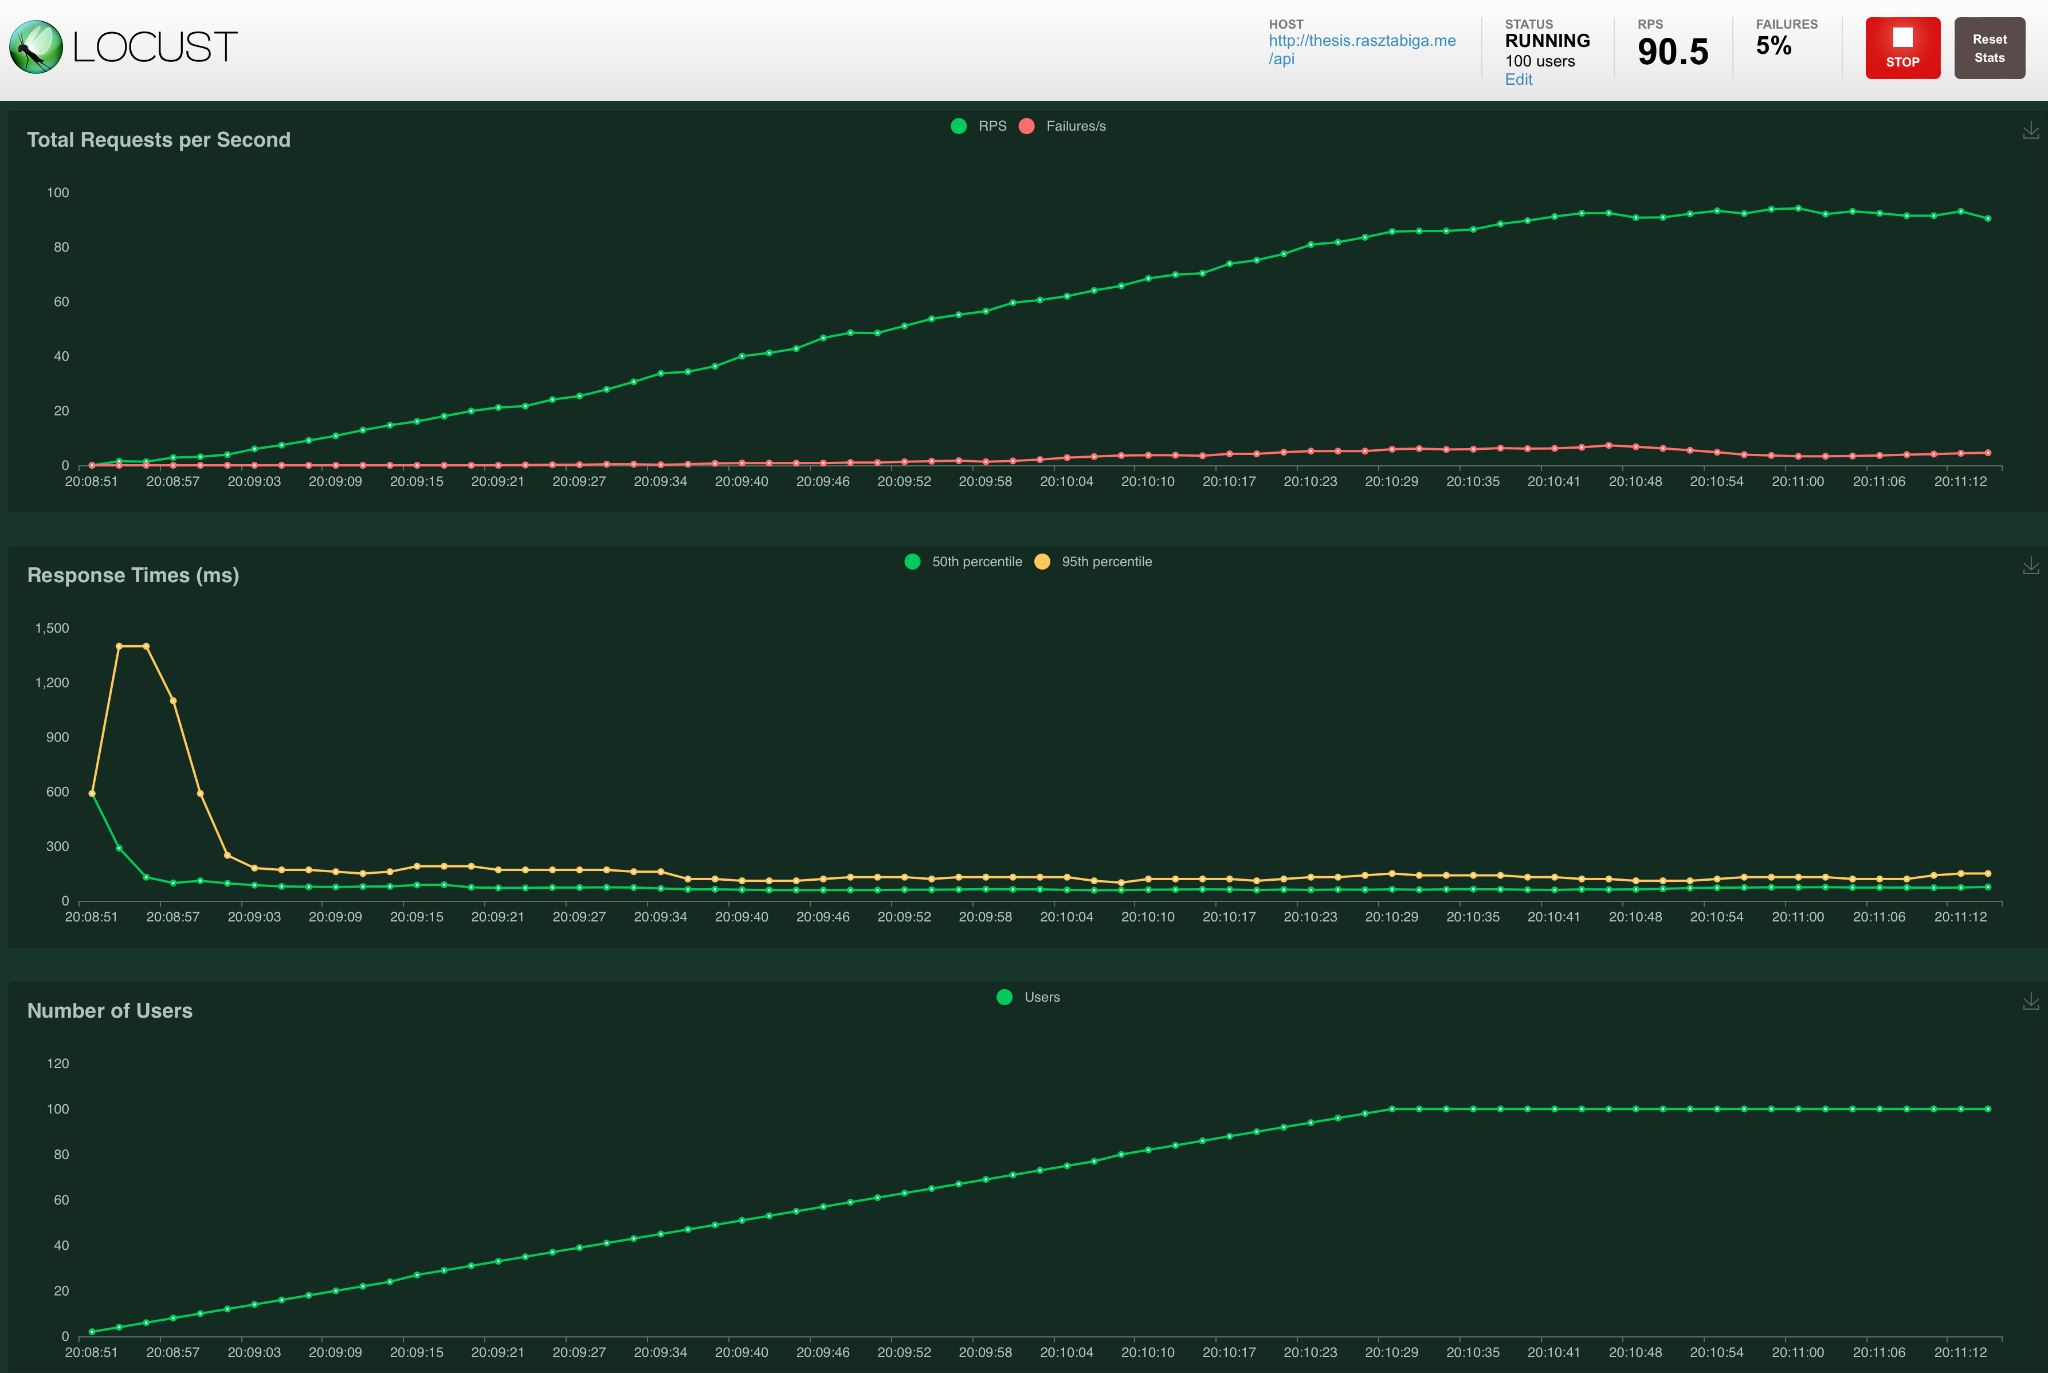
\includegraphics[width=1.0\linewidth]{locust.png}
    \caption{Przykładowy rezultat wykonania testów wydajnościowych}
    \label{fig:locust}
\end{figure}
\clearpage % Rozdziały zaczynamy od nowej strony.

\section{Podsumowanie}

\subsection{Wnioski}

\subsection{Stopień realizacji założeń}

\subsection{Możliwości dalszego rozwoju}

Dalszy rozwój aplikacji, np. w ramach pracy magisterskiej, może obejmować następujące kierunki:

\textbf{Rozszerzenie funkcjonalności aplikacji} W ramach rozwoju aplikacji można rozszerzyć jej funkcjonalność o dodatkowe możliwości, np. analizę i wizualizację danych związanych ze sprzedażą, wydajnością kurierów, itp.

\textbf{Podniesienie wydajności systemu i dalsze testy wydajnościowe} W ramach dalszego rozwoju można podjąć próbę dalszego zwiększenia wydajności systemu, np. poprzez zastosowanie innych technologii, np. innej bazy danych, innych narzędzi do przetwarzania danych, itp. Można również przeprowadzić testy wydajnościowe z wykorzystaniem większej liczby użytkowników równolegle.

\textbf{Ulepszenie warstwy prezentacji części klienckiej} W ramach dalszego rozwoju aplikacji można podjąć próbę ulepszenia warstwy prezentacji części klienckiej, np. poprzez zastosowanie innych technologii, bardziej dopasowanych do dziedziny systemu, takich jak aplikacje mobilne. 

%---------------
% Bibliografia
%---------------
\cleardoublepage % Zaczynamy od nieparzystej strony
\printbibliography
\clearpage

% Wykaz symboli i skrótów.
% Pamiętaj, żeby posortować symbole alfabetycznie
% we własnym zakresie. Makro \acronymlist
% generuje właściwy tytuł sekcji, w zależności od języka.
% Makro \acronym dodaje skrót/symbol do listy,
% zapewniając podstawowe formatowanie.
% \acronymlist
% \acronym{EiTI}{Wydział Elektroniki i Technik Informacyjnych}
% \vspace{0.8cm}

%--------------------------------------
% Spisy: rysunków, tabel, załączników
%--------------------------------------
\pagestyle{plain}

\listoffigurestoc    % Spis rysunków.
\vspace{1cm}         % vertical space
\listoftablestoc     % Spis tabel.
\vspace{1cm}         % vertical space
% \listofappendicestoc % Spis załączników
% \vspace{1cm}
\listoflistingstoc   % Spis listingów

%-------------
% Załączniki
%-------------

% % Obrazki i tabele w załącznikach nie trafiają do spisów
% \captionsetup[figure]{list=no}
% \captionsetup[table]{list=no}

% % Załącznik 1
% \clearpage
% \appendix{Nazwa załącznika 1}
% \lipsum[1-3]
% \begin{figure}[!h]
% 	\centering 
\includegraphics[width=0.5\linewidth]{logopw2.png}
% 	\caption{Obrazek w załączniku.}
% \end{figure}
% \lipsum[4-7]

% % Załącznik 2
% \clearpage
% \appendix{Nazwa załącznika 2}
% \lipsum[1-2]
% \begin{table}[!h] \centering
%     \caption{Tabela w załączniku.}
%     \begin{tabular} {| c | c | r |} \hline
%         Kolumna 1       & Kolumna 2 & Liczba \\ \hline\hline
%         cell1           & cell2     & 60     \\ \hline
%         \multicolumn{2}{|r|}{Suma:} & 123,45 \\ \hline
%     \end{tabular}
% \end{table}
% \lipsum[3-4]

% Używając powyższych spisów jako szablonu,
% możesz dodać również swój własny wykaz,
% np. spis algorytmów.

\end{document} % Dobranoc.
